\documentclass[a4paper, 12pt]{article}

\usepackage{geometry} % Простой способ задавать поля
\geometry{top=25mm}
\geometry{bottom=25mm}
\geometry{left=30mm}
\geometry{right=20mm}

\usepackage{cmap}                
\usepackage{mathtext}         
\usepackage[T2A]{fontenc}
\usepackage[utf8]{inputenc}    
\usepackage[british]{babel}	
\usepackage{rotating}
\usepackage{tablefootnote}
\usepackage{threeparttable}
\usepackage{threeparttablex}
\usepackage{setspace}
\usepackage{amsmath}
\usepackage{tikz}

%\usepackage[paper=portrait,pagesize]{typearea}
\usepackage{subfig}
\usepackage{geometry} % Простой способ задавать поля
\geometry{top=25mm}
\geometry{bottom=25mm}
\geometry{left=35mm}
\geometry{right=20mm}

\usepackage{euscript}     % Шрифт Евклид
\usepackage{mathrsfs} % Красивый
%матшрифт
\onehalfspacing
\usepackage{lscape}

%%% Работа с картинками
\usepackage{graphicx}  % Для вставки
%рисунков
\graphicspath{img/}  %
%папки с картинками
\setlength\fboxsep{3pt} % Отступ рамки
%\fbox{} от рисунка
\setlength\fboxrule{1pt} % Толщина линий
%рамки \fbox{}
%\usepackage{wrapfig} % Обтекание
%рисунков и таблиц текстом
\usepackage{grffile}

\usepackage{csquotes}
\usepackage[style=apa, sorting=nty, bibencoding=utf8]{biblatex}
\addbibresource{citations.bib}
\DeclareLanguageMapping{british}{british-apa}

\usepackage{hyperref}

%\title{Poverty, collective action and politics}

\begin{document}
	    \thispagestyle{empty}
\begin{center}
 \small{ПРАВИТЕЛЬСТВО РОССИЙСКОЙ ФЕДЕРАЦИИ \\
\vspace{4ex}
  ФЕДЕРАЛЬНОЕ ГОСУДАРСТВЕННОЕ АВТОНОМНОЕ ОБРАЗОВАТЕЛЬНОЕ \\
  \vspace{2ex}
  УЧРЕЖДЕНИЕ ВЫСШЕГО ПРОФФЕСИОНАЛЬНОГО ОБРАЗОВАНИЯ \\ 
  \vspace{4ex}
  «НАЦИОНАЛЬНЫЙ ИССЛЕДОВАТЕЛЬСКИЙ УНИВЕРСИТЕТ \\
  \vspace{2ex}
  ВЫСШАЯ ШКОЛА ЭКОНОМИКИ»}
 \vspace{8ex}
 
 \normalsize{\textbf{ФАКУЛЬТУТ СОЦИАЛЬНЫХ НАУК \\}}
 \normalsize{\textbf{ДЕПАРТАМЕНТ ПОЛИТИЧЕСКОЙ НАУКИ \\}}
\end{center}
\vspace{10ex}
\begin{center}
 НОВИКОВ ВЛАДИМИР АЛЕКСЕЕВИЧ \\
 \vspace{4ex}
 \textbf{НЕЧЕГО ТЕРЯТЬ -- НЕЧЕГО ЛОВИТЬ? КАК БЕДНОСТЬ ПОДКРЕПЛЯЕТ ДИКТАТУРУ}\\
 \vspace{4ex}
 \textbf{NOTHING TO LOSE -- NOTHING TO GAIN? HOW POVERTY PERPETUATES DICTATORSHIP} \\
 \vspace{4ex}
 КУРСОВАЯ РАБОТА \\
 ПО НАПРАВЛЕНИЮ ПОДГОТОВКИ 41.03.04 ПОЛИТОЛОГИЯ \\
 СТУДЕНТА ГРУППЫ №181 (ОБРАЗОВАТЕЛЬНАЯ ПРОГРАММА «ПОЛИТОЛОГИЯ»)
\end{center}
\vspace{5ex}
\begin{flushright}
 \noindent
 НАУЧНЫЙ РУКОВОДИТЕЛЬ:
 \\
 КАНД. ЭКОНОМИЧЕСКИХ НАУК, ДОЦ.
 \\
 ЗАХАРОВ АЛЕКСЕЙ ВЛАДИМИРОВИЧ
 \\
 КОНСУЛЬТАНТ:
 \\
 КАНДИДАТ. ПОЛИТИЧЕСКИХ НАУК, ДОЦ.
 \\
 РОЗЕНБЕРГ ДИНА ЯНОВНА
\vspace{5ex}
\end{flushright}

\begin{center}
 \vfill
 МОСКВА -- 2021
\end{center}
	\newpage
	\setcounter{page}{1}
    
    %	\subsubsection*{Abstract}
	
    %\textit{In this paper I study the relationship between the people's poverty and the political regime. I argue that in the static case proportion of population under the poverty line is positively correlated with non-democratic regimes and prolongs their survival. In the presence of the negative income shocks, however the poor are more likely to force the democratic change, which still does not result into the major democratic quality improvements. I also show potential mechanisms which can explain this phenomenon.}
        
        %\subsubsection*{Keywords}
        
        %\textit{Democratization, poverty, authoritarian survival, development, persistence}
        
    \tableofcontents
	
    \newpage
    
    \begin{flushright}
        \textit{We will live normally only when we stop tolerating officials who steal and re-electing them. And if they refuse to hold fair elections, then we’ll take to the streets and remove them from power in this way. This is what distinguishes poor countries from rich ones. In rich countries, people take to the streets at the slightest indignation, and officials are afraid of this. In poor countries, people tolerate all this, and officials hold referendums to extend their powers.} 
        \\
        \vspace{1ex}
        Alexei Navalny, Palace for Putin 
        \\
        \vspace{2ex}
        \textit{Apart from their other characteristics, the outstanding thing about China’s 600 million people is that they are “poor and blank”. This may seem a bad thing, but in reality it is a good thing. Poverty gives rise to the desire for change, the desire for action and the desire for revolution. On a blank sheet of paper free from any mark, the freshest and most beautiful characters can be written, the freshest and most beautiful pictures can be painted}
        \\
        \vspace{1ex}
        Mao Zedong, Introducing A Co-operative
    \end{flushright}
	
	\section{Introduction}
	
	The classical model of autocracy in the academic literature supposes that it is the rule of a few in the interest of a few at the expense of the most \parencite{political_roots, regime_development}. Specifically, it presupposes the so-called <<economic logic of autocracy>> \parencite{handbook}: take money from the poor, give money to the rich. In other terms, dictatorship seems to be the worst possible political regime for the poor. However, we observe that in several non-democratic regimes people who are the main <<losers>> of authoritarianism at the same time appear to be its main supporters, and they sometimes resist change \parencite{more_than_win, prizes}. The topical example might be the higher support of the PRI rule in the poorest counties in Mexico \parencite{voting_for_autocracy} or the grassroots support of the dictatorship in Venezuela \parencite{venezuela}. As there are several case-study papers, this phenomenon still awaits the common theoretical interpretation, support by the cross-national empirical evidence.
	\\
    
	
	\noindent The \textbf{puzzle} here is a lack of actual general theory with an explicit causal mechanism, explaining the interplay between poverty and dictatorship. The \textbf{research question} is: how does the people's poverty affect political institutions to prolong authoritarian survival? And the \textbf{subject matter} -- social and economic origins of the political regimes.
    \\\\
    This problem is important for the following reasons: (a)  some states (China, Vietnam, etc.) kept authoritarian rule (or authoritarianized: post-Soviet regimes) and reduced poverty; (b) poverty decreased, but affected institutions might persist; (c) in recent years we observe both the authoritarian backlash and likely poverty increase due to the economic crisis; (d) poverty still persists in some parts of the world (Africa, Latin America, South-Eastern Asia) and massive poverty reduction requires too much of an economic growth \parencite{povertyend}.
    \\
    
    \noindent The proportion of the world's population under all poverty lines reduced significantly in the last 30 years \parencite{wbpoverty20} partially due to the <<War on Poverty>>. At the same time there became fewer authoritarian regimes due to the Third wave of democratization. These facts appear to be connected as poverty reduction is correlated with democratization \parencite{poverty_democratization}. Nonetheless, poverty still persists \parencite{poverty_persistence} in certain countries (especially in Central Africa) and so does dictatorship \parencite{vdem, poverty_interplay}. And what is even more challenging, poverty reduction in certain countries did not result in democratization, consider China, Vietnam, or Post-Soviet states \parencite{autocratic_middle}. The Figure \ref{fig:pol_pov} have four subplots\footnote{Left column shows the proportion of the population under the \$1.9 international poverty line while the right one -- Polity IV score. The top row shows the first occurrence of either poverty or polity measure after 1991 and the bottom row -- the latest one} and illustrates all the fluctuations described above.
	\\
	%\begin{landscape}
	\begin{sidewaysfigure}
	%\begin{figure}[!h]
	    \centering
	    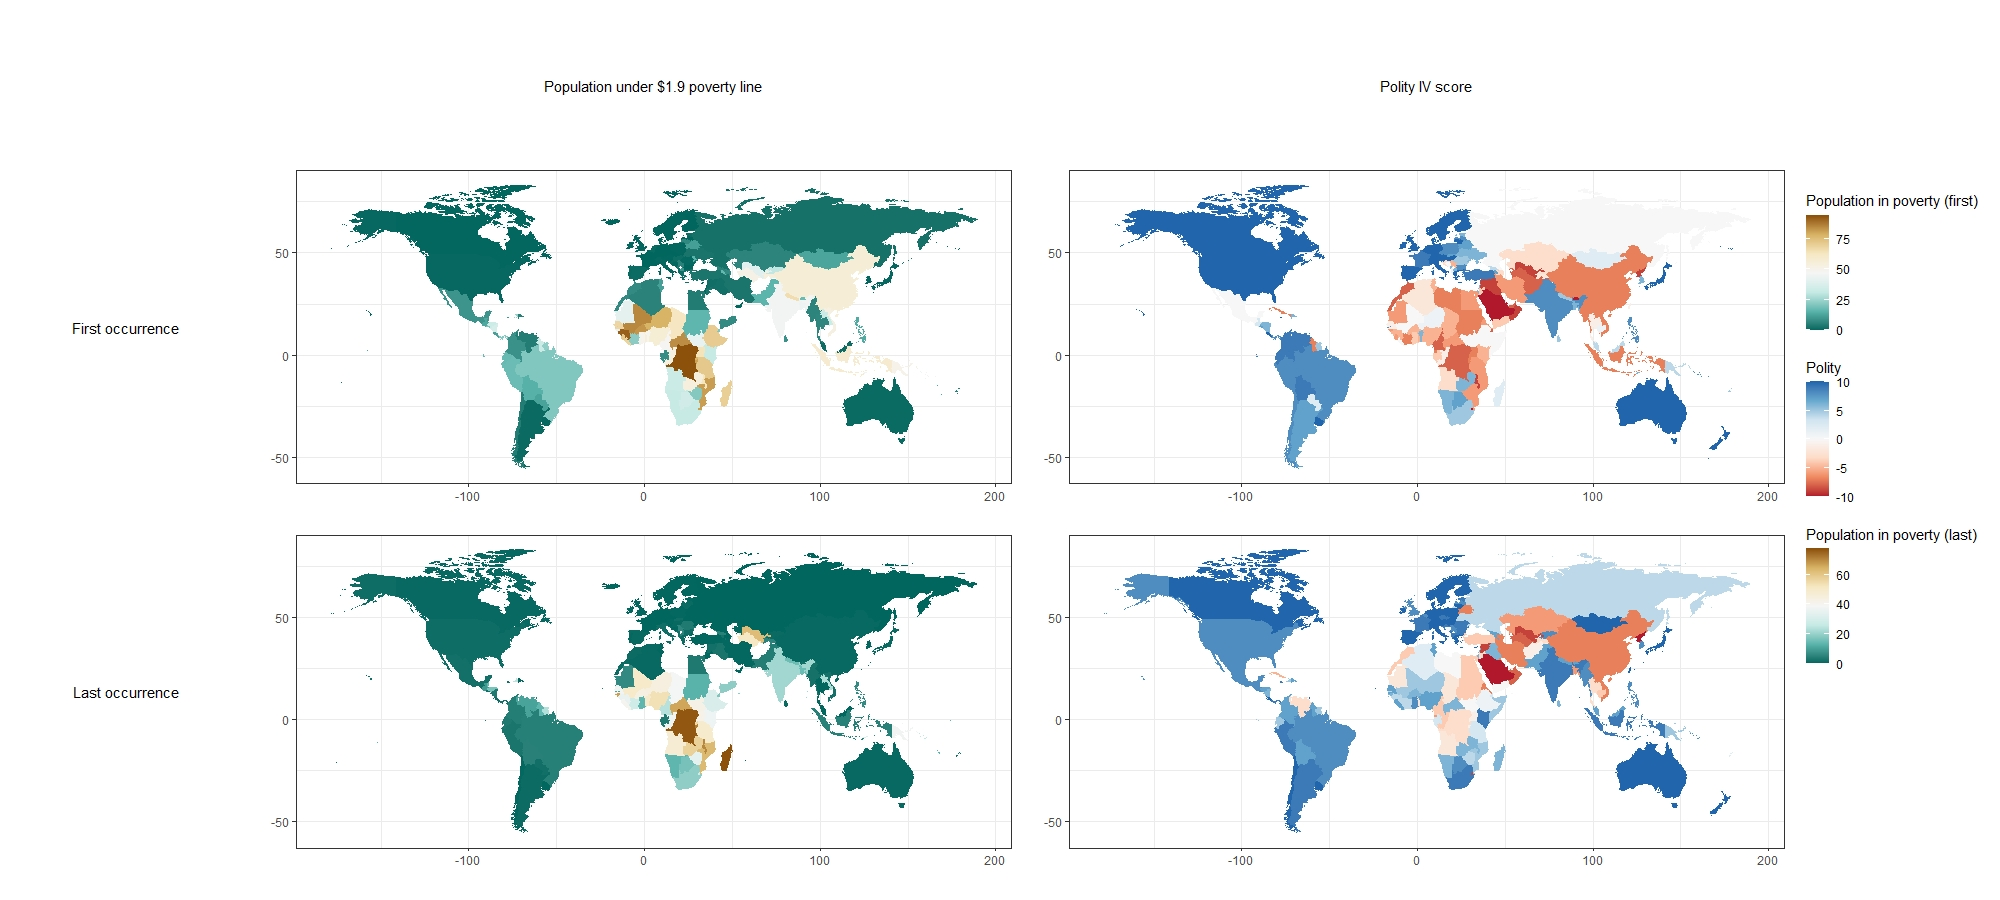
\includegraphics[width=26cm]{img/pol_pov.jpeg}
	    %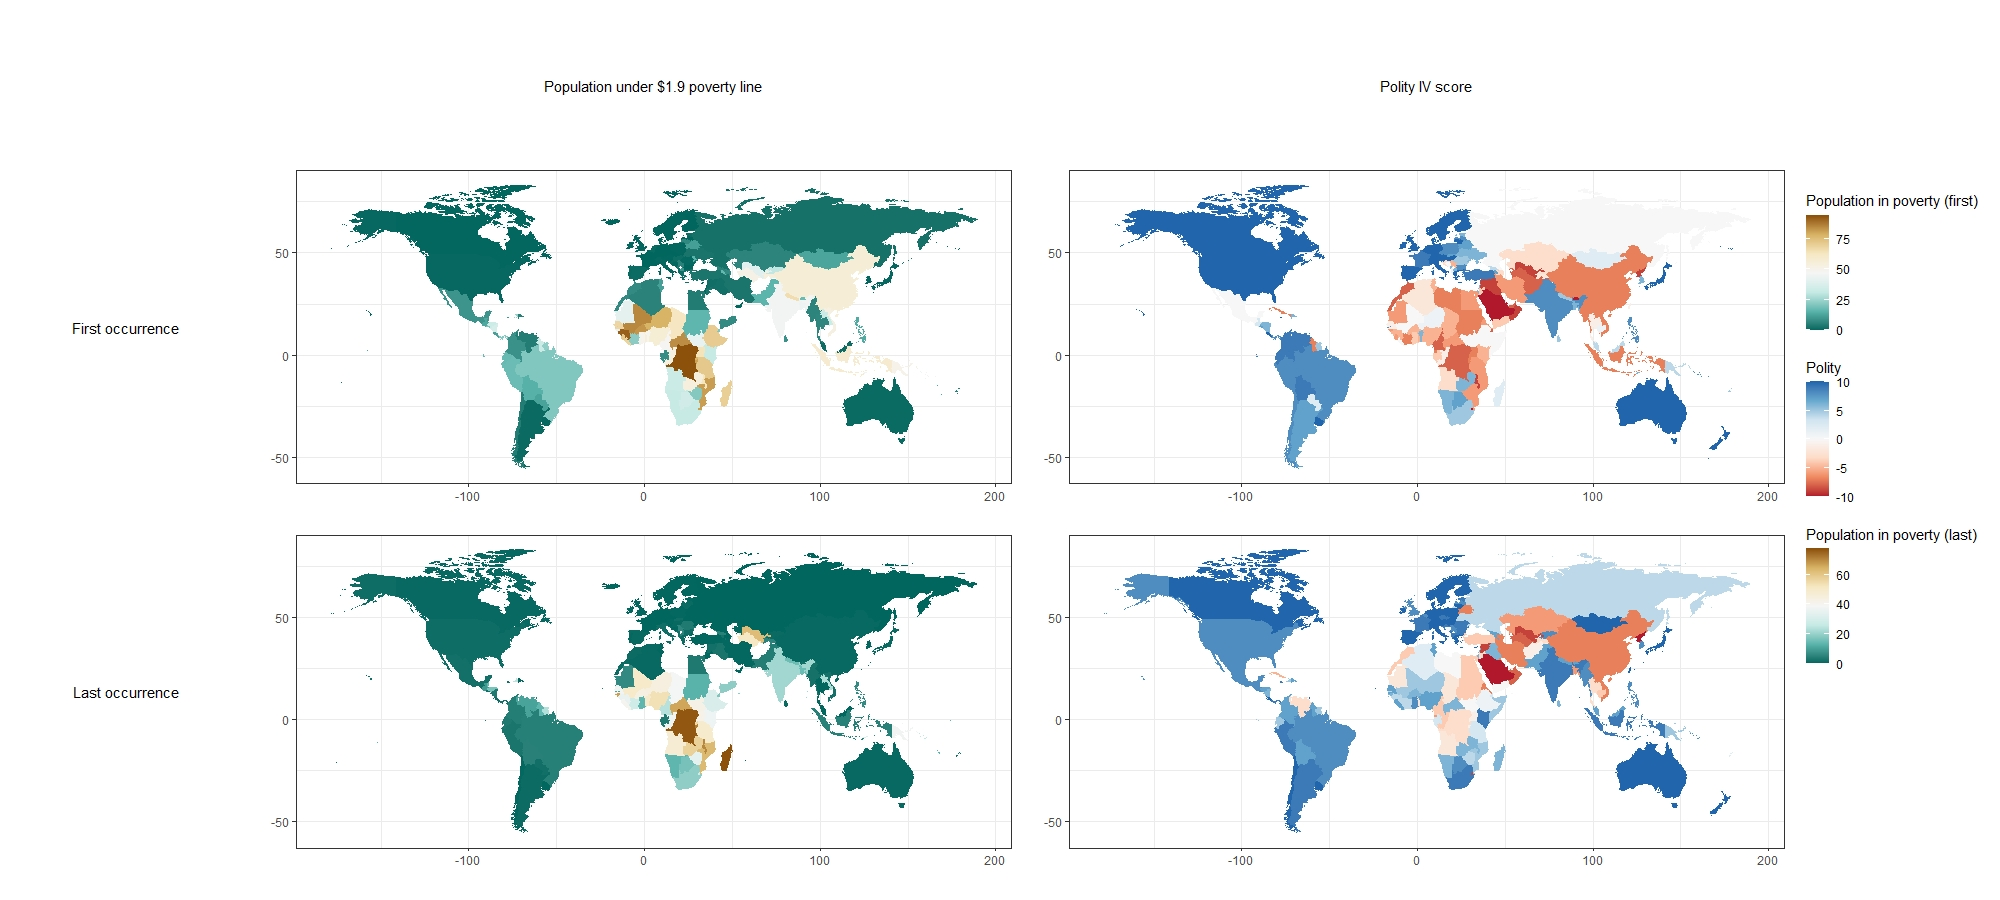
\includegraphics[angle=90,width=10.35cm]{img/pol_pov.jpeg}
	    \caption{Poverty and political regimes after 1991}
	    \label{fig:pol_pov}
	%\end{figure}
	\end{sidewaysfigure}
	%\end{landscape}
    
    \noindent The \textbf{goal} is the analysis of the effect of poverty on authoritarian persistence and the mechanism of such influence. To achieve this aim there are the following \textbf{research tasks} to do: (a) create a formal theoretical model, explaining the impact of poverty (and its implications) on the political regime; (b) empirically verify the model's predictions; (c) check the robustness of the empirical investigations (d) test the proposed mechanism.
    \\\\
    To resolve these objectives, I abide by the rational choice \textbf{methodology}. I imply limited rationality of the agents and model their strategic choices. I also utilize the following \textbf{methods}: game-theoretical formal modeling and a bunch of statistical methods, including panel data analysis, conditional and Bayesian logit models, two-step least-squares regressions, and the causal mediation analysis.
	\\\\
	The paper is organized as follows: the next section presents the literature survey and the theoretical framework of the paper, after that in the third section I introduce the formal model of income and political revolution and finalize theoretical propositions. The following section 4 contains descriptions for the data and the empirical methods and section 5 shows the results of the statistical analysis. In the next section 6, I check the robustness of the empirical results, and in section 7 I propose and empirically test the causal mechanism. In the last sections 8 and 9, I reinterpret the results in the broader context, provide some illustrations for my theory, and conclude.
	
	
	
	
	
	\section{Existing Research and Theoretical Framework}
	
    In this section, I present the theoretical approach of this paper which presumes that the political structure of the society is driven by social and economic conditions. Next, I look more precise on the reasons why poverty and, consequently, the poor are amiss for democracy. The main features are a lack of social capital, displaced inter-temporal preferences, and a lower ability to commit to collective action. Finally, I look at the conditions which allow the poor to cooperate and overthrow the status quo.
	
	\subsection{How Social Structure Affects Politics}
	
	The idea that a political shape is affected by the social and economic structure of the society has been spoken since Aristotle's Politics \parencite{aristotle}. He was the first one to declare that the very specific anthropological type -- the \textit{Golden mean} (prototype of the future Middle class) -- is the necessary condition of a democratic society. Since then the various scholars, mostly working within the liberal framework were developing the concept of the very concrete social group, which is interested in the liberal and democratic government and political institutions, which broaden political participation. This is also a source for a theoretical framework for the analysis of the numerous democratic revolutions, from the Glorious Revolution in 1688 to the latter, and the very recent fall of the Soviet Union and Arab spring were analyzed using this framework. A kind of different interpretation was provided by the famous Marxist analysis of politics, as the superstructure above the economical basis of the society, i.e. the class relations \parencite{marx}. Still, most of the modern political economy studies are based on his thesis that political conflicts could be explained using economic relations.
	\\\\
	One of the most notable classical works on the past revolutions, which lead either to the democracy or another dictatorship was done by Barrington Moore Jr. \parencite{social_origins}, who presented his analysis of six different revolutions which resulted in different outcomes with different costs. He claimed that the variation in the outcomes and costs could be explained by the balance of the social forces and their economic relations within the society. His main idea can be simplified to the thesis \textit{<<no bourgeois, no democracy>>}. It is more or less clear why the landowning aristocracy is not interested in democratization, but why should the peasants be supporters of the \textit{Ancien Régime}? In Moore's logic, democratization and modernization are parts of the same process (and peasants are parts of the pre-modern world). And what about the modern world wherefore the poor do not suit the democracy? 
	\\\\
	Newer studies are developing the idea of socio-economic origins of the political order: multiple works by Acemoglu, Robinson, and co-authors did in the framework of new institutionalism are build upon the idea that institutions, which connected with the distribution of power within the society, are the product of social forces \parencite{inst_per}. Thus, democratization is just a matter of the game between the elites and the people \parencite{econ_origins}. Worth mentioning, that the probability of democratization increases as the Middle class is added to the model. What about the poor: the book presents the very Marxist idea that if people are poorer, they have lesser to lose, and thus they are more likely to revolt. However, their next work \parencite{why_fail} develops the idea that institutions themselves affect the quality of governance and policy outcomes and also describes more complicated cases of the persistence of inefficient government: the people gain less than they would under another government and institutions, but it manages to stay robust. The complicated question of persistence was studied in another paper \parencite{gov_pers} and is also the matter both of the balance of the social forces and the current institutional equilibrium. It is also useful to mention one more time that the political outcomes and the overall political shape of the society are all the product of the social structure via the institutions, which capture the distribution of power within the social group. And democracy highly depends on the contention and struggle between the society and state and within the society \parencite{corridor, contention}.
	\\\\
	That is the general theoretical framework this paper is following. To summarize: the political landscape is rooted in the socio-economic structure of the society, i.e. the specific shape of the so-called classes. For democracy, the vital conditions are the large middle class and the constant struggle. Whereas, numerous people in poverty and institutional stasis are the unsafe conditions likely to lead towards the democratic decline.
	
	\subsection{Consequences of Poverty}
	
	But why scholars assume poverty is hazardous for democracy? In this part, I review several implications of poverty on human behavior. First, it is studied that absolute or extreme poverty, so-called, scarcity, affects people's decision-making so that they act irrationally. That is because people in scarcity have biased inter-temporal preferences, as their consumption in the present is so low that they rate it much higher than more secure people. And that is the reason why they dismiss long-distance goals in favor of short-term benefits \parencite{scarcity, poverty_consequences}. That is a substantial notice and one of the key assumptions of this paper: the poor value present consumption relatively higher to the future compare to the Middle class and the elites. A complex study of the interplay between the poverty of the population and the non-democratic politics in Africa also shows that the poor are vulnerable for the short term benefits, and thus they are less likely to support the long term potentially more profitable policies \parencite{poverty_interplay}. There is also evidence that the income affects the people's regard to the success in their life: more wealthy people tend to attribute the achievements to their dignities and their failures to bad luck and the limitations of the system while the poor on the contrary attribute their achievements to the external circumstances and their failures to their personality \parencite{poverty_ideology}. This also implies that more wealthy people are more likely to attempt to achieve their goals and more likely to believe in their pivotalness. That is also connected with attitudes to risk and studies show that the poor tend to be more risk-averse compare to the more well-being people \parencite{poverty_risk}.
	\\\\
	Moreover, poverty also affects the social incentives and attitudes: poverty can negatively affect the social trust \parencite{trust_poverty2} thus lowering social capital. At the same time trust within the local community can affect the discussed above <<myopia for the future>> and thus contribute to the poverty persistence \parencite{trust_poverty}. Furthermore, the understanding of poverty should not be limited by economic poverty but should include social poverty too as it is more connected with trust \parencite{trust_poverty3}. An empirical study from China and Bangladesh also shows that social capital is crucial for economic development, well-being and overcoming poverty, visa-versa lack of social capital is associated with poverty persistence \parencite{poverty_capital, poverty_capital2, poverty_capital3}. And numerous studies are explaining why and how social capital is essential for democracy. The defining book is Olson's <<Logic of the collective action \dots>>, where he stated that the social capital is one of the instruments to solve the collective action problem \parencite{collective_action}. Afterward, the classical books by Putnam showed that variation in social capital explains the variation in the quality of democracy in Northern and Southern Italy \parencite{italy_capital, bowling} to more recent works \parencite{social_capital_democracy} coming with the same claim: social capital and generalized social trust are fuelling associations and lower-level democratic institutions which in turn are oiling the democracy at the state level.
    
    \subsection{Poverty and Inequality}
    
    \noindent However, not just poverty itself or absolute poverty might affect the preferences of the poor and push them to support the dictatorship. Numerous studies show that indeed relative feel of wealth and relative poverty might change the people's attitudes towards power and authority and thus lead to the dictatorship \parencite{relative_power}. The same ideas about income inequality and interconnection with non-democratic preferences and politics have been developed in a different paper, which shows that economic inequality causes political inequality \parencite{inequality_regimes}. However, other scholars suppose there might be a more complex relationship between inequality and authoritarian politics \parencite{regime_inequality} and sometimes demand redistribution might lead to democratization \parencite{inequality_democracy}.
	
	\subsection{Political Regime and Socio-economic Performance}
	
	The relationship between the political regime and economic performance is one of the greatest challenges for both political scientists and economists. The evidence is sometimes contradictory, so this topic will concentrate more on the studies that outline the theoretical framework this paper is following. The defining study in this field might be Olson's work \parencite{regime_development}. He proved, using formal modeling and basic empirical analysis, those authoritarian regimes can provide only short-term economic growth due to information constraints and uncertainty, while democracies are showing way better results. The idea is further developed as it was proved with more complicated statistical analysis that democracy (however with enough state capacity) is crucial for the economic development \parencite{regime_development_2}. The classical work by Przeworski and co-authors \parencite{democracy_development} discovers using large longitudinal empirical data set that after reaching a certain level of income (slightly more than \$ 6000 per capita) democratic regimes are less likely to die and more likely to survive as democracies. Whereas, dictatorships follow a different pattern as they are most likely to survive either if income is very low (under \$ 1000) or very high (more than \$ 7000). And the medium income level is the most dangerous one for the non-democratic regimes.
	\\\\
	Several studies support these findings, but with a few different results, there is evidence that economic performance is crucial for the survival of the democratic regimes while the dictatorships are almost non-dependent on their economic conditions \parencite{hazard_rate}. That might happen as at the competitive elections in the developing countries voters are more likely to punish rulers for bad social and economic performance and recessions rather than to support them for reasonable results \parencite{econ_vote}. And dictatorships are less dependent on popular vote and public support \parencite{inst_surv}. The idea that democracies are more dependent on economic conditions is also developed in an alternative way, as Acemoglu and co-authors argue that democratization causes economic growth to compare to stable authoritarian status-quo \parencite{democracy_growth}. A kind of opposite logic is developed by a study of public goods provision after the regime change \parencite{regime_public_goods}. Right after the transition non-democratic regimes provide more public goods compare to democracies, but they decrease the provision with time while democracies follow the opposite trend. It means that after the dictatorship consolidates and institutionalizes it is less dependent on public goods provision, economic conditions, and co-optation. Yet but by different means dictatorships might be interested in economic growth and can even create some democratic institutions which constraint dictators and reduce uncertainty \parencite{inst_constr, why_parties}. Still, the authoritarian regimes are less likely to contribute to social welfare from that growth as other studies show that democracies are showing better social performance \parencite{regime_performance} and democracies are more likely to decrease income inequality \parencite{regime_inequality}. 
	
	
	\subsection{Poverty and Non-Democratic Politics}
    
    But why it happens so that dictatorships are conceding in terms of economic and social performance but still manage to survive? Several studies conducted by De Mesquita aim to find the causal roots of poverty in the specific economic logic of authoritarian politics \parencite{political_roots}. The thesis is that this logic can be described as reversed Robin Hood, i.e. <<take money from the poor and give money to the rich>>. The logic behind this is connected with the concept of selectorate which stands for the group of people who is able to select the leadership. In order to stay in power, the leader needs to provide some goods for the selectorate and as democracy has the broadest selectorate (almost the whole population) democratic leaders have to provide public goods and care about the well-being of a large coalition of supporters. Meanwhile, in the dictatorship by the definition of selectorate is as thin as possible, and as long as the dictator manages to elaborate the specific group of high-ranking supporters and the army he should only care about their well-being while the welfare of all the other people is irrelevant for his political survival \parencite{handbook}.
    \\\\
    But why the poor should support such a regime? Case study of the Mexican The Institutional Revolutionary Party (or PRI) rule throughout the XX century by Magaloni \parencite{voting_for_autocracy} aims to answer this question. The challenge was that the PRI gained the highest electoral support in the poorest counties in Mexico, in the regions which were the main losers of that regime. Magaloni figured out that this happened due to large co-optation politics and specific prizes for voting for PRI during the electoral cycle. Co-optation is one of the main survival strategies in the dictator's toolkit, in line with the repressions and legitimation, which helps to remain in power and to stabilize the regime \parencite{three_pilars, toolkit}. As it was mentioned above, sometimes with the aim of achieving economic growth authoritarian regimes establish elections and co-optation is the instrument to mobilize the electorate to vote for the regime or just to use rallies as a signal \parencite{regional_roots, mobilization}. Co-optation is mostly achieved via the distribution of the specific prizes for the supporting groups. There are two important notes connected with these patronage practices: first, to get the prizes, social groups might organize and even falsify the election results themselves \parencite{more_than_win} to show their support. Second, smart politics of co-optation and specific perks for apparent pivotalness of the support might make some social groups support the policy which is in long run unprofitable for them intending to get prizes in the short run \parencite{prizes}. A suggestive conclusion that the poor are the most susceptible to this kind of politics is supported by the empirical inference from Latin American regimes \parencite{patronage}.
	
	\subsection{How to Break Through}
	
	Nevertheless, under specific circumstances, the people mired in poverty are able to start an uprising and succeed. These episodes are studied via the paradigm of \textit{windows of opportunity}. These conditions are mostly achieved due to the external shocks, which can break the status quo, mostly negatively affecting the state of affairs. And because of these negative external shocks people, who have sometimes literally nothing to lose, rise in revolt. Remarkable papers that come after this approach are the following. In both articles, Brückner and Ciccone \parencite{oil_dem, rain_dem} estimate how negative economic external shocks affect democratization. Their logic is as follows: either oil price shocks (for oil-producers countries) or the massive rains (in Sub-Saharan agrarian Africa) result in economic crises, which affect the people's income. And next to the people uprise and overthrow the current government: they measure the democratic transition via the change in Polity IV score. Their empirical methods are also notable as they use Instrumental Variables to draw the causal inference. Other recent studies draw democratization as a two-step process, starting from an exogenous shock causing popular uprising and continued (or not) by the new political elites \parencite{shockdemoc}. However, other researchers argue that the effect of economic shocks is dependent on the role of the state in the economic structure of the society as higher state engagement makes it more vulnerable for the crises \parencite{crisisdemoc}.
    \\\\
	Their outcomes stand in line with the previous study in the field, as the external shocks are studied as the trigger for the revolt \parencite{social_origins, econ_origins}. While the causes might be rooted deep in the social and economic factors, without the rare events, discarding the current institutional shape, the status quo may persist. An optimistic (from pro-democratization point of view) finding might be that as absolute poverty reduces in recent decades, it leads to a slow yet steady and robust trend to democratization \parencite{poverty_democratization}.  
	
	\section{Formal model}
	
    Consider the state with the set of $N \in \{1, 2, \dots n\}$ citizens of two types: with $\tau_i = L$ (Low) or $\tau_i = H$ (High) income. $S$ is the share of the citizens with the Low income, i.e. there are $S \cdot N$ such individuals. Each citizen chooses between three actions $a_i \in \{r,s,c\}$ where $r$ denotes "revolt", $s$ "stay at home" and $c$ "co-opted by the regime".
    \\\\
    \noindent Let's denote by $t$ the threshold for the amount of citizens choosing to "revolt" for the revolution to succeed (i.e. $\# \{j \in N: a_j = r\} \geq t$), otherwise the dictatorship remains. I suppose, following \cite{enterpreneurs} and \cite{overthrowing} that the value of $t$ is the public information.
    \\\\
    \noindent I suppose that revolting is associated with additional costs $-c$ compare with staying at home (i.e. $U_{r} = U_s-c < U_{s}$ if all others equal) while being co-opted increases the utility by $p$ (i.e. $U_{s} < U_s+p = U_{c}$ with all others equal). The first assumption is common for the collective action models and can be interpreted as the risk of punishment or violence during the revolt (or if the revolt fails) and the second one comes from the literature as being co-opted often means gaining certain "prizes" \parencite{voting_for_autocracy}. I also suppose that all the citizens benefit from the revolution regardless of whether they participated or not (that is, all citizens receive payoff $P$) and taking into account the citizens action the result if the revolution succeeds is the following: $U_{r,R} = P - c<U_{s,R} = P < U_{c,R} = P +p$ (with $U_R$ corresponding to the utility if the revolt succeeds).
    \\\\
    Finally, I assume that the benefit from revolt is delayed (as the revolt is the lasting process), thus the utility is discounted, specifically, $\delta P$ instead of simply $P$. As the literature suggests, the discount value might vary with discount being higher for the ones with high income ($\delta_H > \delta_L$, thus, the ones with high income value future utility higher). Thereby, for the citizens with high income $\tau_i = H$ benefit of being co-opted is lower than the potential gain of successful revolt ($p < \delta_H P - c$) and the utilities are as follows $U^H_{r,F}<U^H_{s,F}<U^{H}_{c,F}<U^H_{r,R}<U^H_{s,R}<U^H_{c,R}$ (where $U_F$ -- stands for the utility if the revolution fails). However, for the citizens with the low income, $\tau_i=L$ due to the lower discount value (i.e. biased time preferences) and because the same prize for co-optation has higher relative benefit ($c > \delta_L P - p$) the utilities are the following $U^L_{r,F}<U^L_{s,F}<U^L_{r,R}<U^{L}_{c,F}<U^L_{s,R}<U^L_{c,R}$.
    \\\\
    Note, that for both types of citizens being co-opted strongly dominates staying at home: with both strategies, the citizen does not participate in the revolt, but in the first, he gains an additional prize for co-optation. So I can exclude the latter from the analysis and focus on the choice between being co-opted and revolting with the following utilities:
    \begin{subequations}
    for type $\tau_i=H$
    \begin{equation}
        U^H_{r,F}<U^{H}_{c,F}<U^H_{r,R}<U^H_{c,R}
    \end{equation}
    And for type $\tau_i=L$
    \begin{equation}
        U^L_{r,F}<U^L_{r,R}<U^{L}_{c,F}<U^L_{c,R}
    \end{equation}
    \end{subequations}
    \\
    \noindent Also note that in such scenario the citizens with the low income basically never choose to revolt as for them $U^L_{r,R}<U^{L}_{c,F}$.
    \\\\
    \noindent Then I study two cases: the baseline with the setup described above and the revolution in presence of an exogenous income shock, which reduces the regime's ability to co-opt citizens.
    
    \subsection{Solution}
    
    \begin{quote}
        \textbf{Proposition 1} \textit{If $N - S\cdot N < t$ there is no revolution in equilibria.}
    \end{quote}
    
    \noindent That is the obvious proposition, because regardless of whether $S$ is the public or private information even if all the citizens with high-income revolt it will not be enough for the revolution to succeed, and as it was stated above for the poor it is more beneficial to be co-opted compare to participating even in the successful revolt.
    
    \begin{quote}
       \textbf{Proposition 2} \textit{If $N-S\cdot N \geq t$ there are multiple equilibria}.
    \end{quote}
    
    \noindent This is common multiple equilibria result in the coordination games. Since for the citizens with the high income the revolution is more beneficial, there are two possible outcomes: (1) nobody revolts if the citizens with high income do not believe that the others would revolt (or if case when $S$ is the private information they suppose that there are not enough citizens with the high income) (2) multiple equilibria with the exactly $t$ citizens with high income choosing to revolt if they believe that there are enough other citizens of type $\tau_i = H$ who choose $a_i = r$. 
    
    \subsection{Income shock}
    
    Now, let assume that the negative exogenous income shock happens, which reduces the citizens' income, but does not affect their utility if the revolution succeeds (that is the reasonable assumption as we can interpret the benefit from the revolution as the redistribution of the dictator's personal income, property, and estate which is less vulnerable for the economic fluctuations). So the newer utilities are the following:
    \begin{subequations}
    for type $\tau_i=H$
    \begin{equation}
        U^{H, shock}_{r,F}<U^{H, shock}_{r,R}<U^{H, shock}_{c,F}<U^{H, shock}_{c,R}
    \end{equation}
    And for type $\tau_i=L$
    \begin{equation}
        U^{L, shock}_{r,F}<U^{L, shock}_{c,F}<U^{L, shock}_{r,R}<U^{L, shock}_{c,R}
    \end{equation}
    \end{subequations}
    
    \noindent Now the situation is the opposite, as it is beneficial for the citizens with the low income to participate in the successful revolution (as their income aftershock is that low that even if they are co-opted it is less, that they gain after the revolt). On the contrary, for the citizens with a high income being co-opted is now profitable to be-opted than participate in the unsuccessful revolt.
    
    \begin{quote}
        \textbf{Proposition 3} \textit{In presence of shock if $S\cdot N \geq t$ there are multiple equilibria.}
    \end{quote}
    
    \noindent It is again the multiple equilibria result in the coordination game, but now the citizens of type $\tau_i = L$ are the momentum of revolution. So there are two sets of outcomes: (1) nobody revolts if the citizens with the lower-income do not believe that the others would revolt or do not know if there are enough citizens of such type (2) exactly $t$ citizens of type $\tau_i = L$ choose to revolt if they believe that the others would do so.
    
    \begin{quote}
        \textbf{Proposition 4} \textit{In presence of shock if $S\cdot N < t$ there is no revolution in equilibria.}
    \end{quote}
    
    \noindent Obviously, now the citizens of type $\tau_i=H$ never choose to revolt, so there are not enough possible revolutionists.
    
    \subsection{Implications and Empirical Hypothesis}
	
	To sum up the implications from the formal model, there are two main findings: (1) In the "static" case (with no income shock) the higher proportion of the citizens with low income (higher S) reduces the probability of revolt as it is either no possible revolt at all (in case of $N - S\cdot N < t$) or reduces the number of possible combinations of individual strategies, resulting in revolt (in case of $N - S \cdot N \geq t$ we have multiple equilibria with exactly $t$ citizens of type $\tau_i=H$ choosing to revolt, with a higher proportion of $S$ we have a lower number of such combinations); (2) In presence of an exogenous income shock higher proportion of poverty, on the contrary, reduces the probability of the revolution: if $S\cdot N < t$ the revolt is impossible if $S\cdot N \geq t$ with the increasing $S$ there is the higher number of combinations of citizens of type $\tau_i=L$ such as $\# \{j \in S \cdot N: a_j = r\} = t$.
	\\\\
	\noindent Or, in other words, the following empirical hypotheses could be drawn:
	\begin{quote}
	    \textbf{Hypothesis 1} \textit{States with higher levels of poverty are less democratic}
	    \\\\
	    \textbf{Hypothesis 2} \textit{Higher levels of poverty has a lower probability of the authoritarian regime breakdown}
	    \\\\
	    \textbf{Hypothesis 3} \textit{In presence of an exogenous income shock higher levels of poverty result into the democratization process}
	\end{quote}
	
	\noindent In addition to the direct implications of the model, there is one more proposition to be drawn. After the income shock happened, and its effect nullified economic conditions in society return to the status quo. Or, in other words, the window of opportunity closes. Thus, the game returns to the initial setup with the higher proportion of citizens with Low income decreasing the probability of revolt, which could be interpreted in terms of potential to control the government. Thereby, there is the last hypothesis:
	
	\begin{quote}
	    \textbf{Hypothesis 4} \textit{Higher poverty rates can hinder the democratizing effect of an exogenous income shock}
	\end{quote}
	
	\section{Data \& Methods}

	\subsection{Empirical Strategy}
	
	I incorporate the branch of statistical techniques to test empirically the hypotheses proposed above. To test the <<static>> scenario I utilize ordinary least squares model with fixed effects to test the relationship between poverty and political regimes. 
	\begin{equation}\label{plm}
	    d_{i, t+k|k\in\{1,5\}} = \beta p_{i,t} + \sigma w_{i,t}+\mu_i+\tau_t +\varepsilon_{i,t}
	\end{equation}
	\noindent Apart from that, I apply the two-step least squares models to test for possible causality with negative income shock as an exogenous instrument for poverty in the auxiliary regression:
    \begin{subequations}\label{eq:2sls}
    \begin{equation}
        p_{i,t} = \gamma s_{i,t-m|m\in\{0,3\}} + \sigma w_{i,t}+\mu_i+\tau_t +\varepsilon_{i,t}
        %\tag{\ref{eq:2sls}}
    \end{equation}
    Fitted values from the equation above are used as a predictor for the political regime measure:
    \begin{align}\label{2sls2.1}
        d_{i, t+k|k\in\{1,5\}} = \beta \hat p_{i,t} + \sigma w_{i,t}+\mu_i+\tau_t +\varepsilon_{i,t}
    \end{align}
    \end{subequations}
	\noindent Where $d_{i, t+k|k\in\{1,5\}}$ is a regime measure in a country \textit{i} in periods $t+k$. $s_{i,t-m}$ stands for a binary variable for a negative income shock in country \textit{i} in periods $t-m$ and  $p_{i,t}$ -- poverty estimate in a country \textit{i} in period $t$. $w_{i,t}$ stands for a vector of controls and $\mu_i, \tau_t$ are country and time fixed effects, with the first ones removed by the within transformation.
	\\\\
	\noindent To check the survival hypothesis I use the binary response model with authoritarian regime failure response and poverty estimate as an explanatory variable. I make use of both conditional logit, as it accounts for the heterogeneity within the data:
	\begin{equation}\label{logitfail}
	    P(y_{i,1}\dots y_{i, n_i} | \sum_{j=1}^{n_{i}} y_{i,j} = k_{1,i}) = \dfrac{\exp ( \sum^{n_i}_{j=1} y_{i,j} \cdot (\beta p_{i,t} + \sigma w_{i,t}+\mu_i+\varepsilon_{i,t})) }{\sum_{d_{i} \in S_{i}} \exp(\sum^{n_i}_{j=1} y_{i,j} \cdot (\beta p_{i,t} + \sigma w_{i,t}+\mu_i+\varepsilon_{i,t})})
	\end{equation}
	\noindent And linear probability models as for the rare event data if the response gets positive value in 25\% cases or less frequently (and authoritarian breakdowns take place in 4.7\% cases and regime changes as such in just 1.4\% cases, see Figure \ref{fig:pol_hists}) linear probability model is preferable to the logit \parencite{lpm}:
	\begin{equation}\label{lpm}
	    ab_{i,t} = \beta p_{i,t} + \sigma w_{i,t}+\mu_i+\tau_t +\varepsilon_{i,t}
	\end{equation}
	
	\begin{figure}
        \centering
        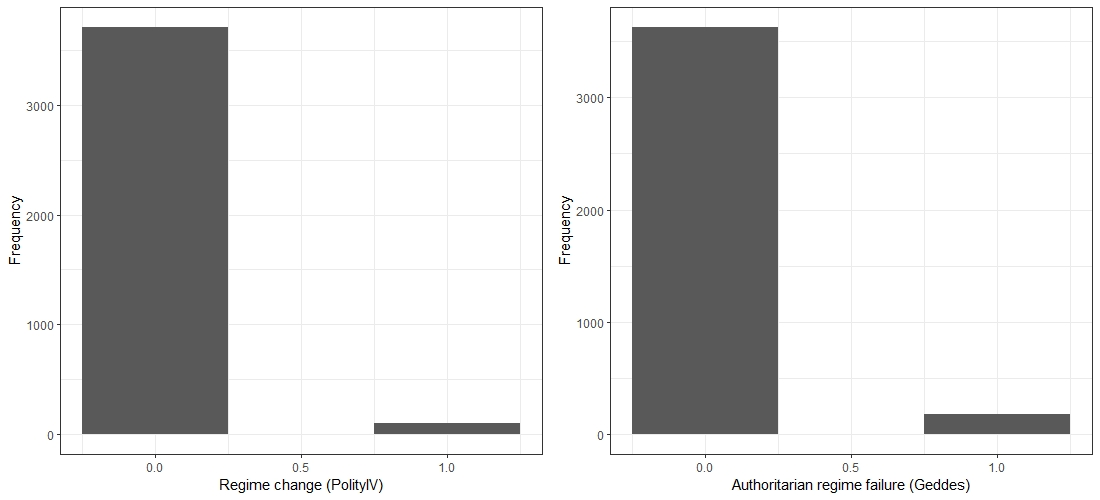
\includegraphics[width=\textwidth]{img/pol_hists.jpeg}
        \caption{Regime breakdowns distributions}
        \label{fig:pol_hists}
    \end{figure}
	
	\noindent Where $ab_{i,t}$ stands for the binary measure for the authoritarian breakdown in a given country \textit{i} in year \textit{t}, i.e. whether the political regime classified as dictatorship in a given country failed in a particular year. $p_{i,t}$ -- poverty estimate in a country \textit{i} in period $t$. $w_{i,t}$ is a vector of controls and $\mu_i, \tau_t$ are country and time\footnote{Note that the logit model does not include the time fixed effects, as otherwise the model fails to converge} fixed effects.
	\\\\
	\noindent As a placebo test whether the effect of poverty is identical or different for democratic and non-democratic political regimes I include the interaction effect between the binary democracy-dictatorship indicator and poverty estimate in the model. Note that now the regime change as such, not just authoritarian breakdown is the response variable:
	%\begin{subequations}
	\begin{equation}\label{lpmchange}
	    rc_{i,t} = \beta p_{i,t} + \eta DD_{i,t} + \gamma [p_{i,t} \cdot DD_{i,t}] + \sigma w_{i,t}+\mu_i+\tau_t +\varepsilon_{i,t}
	\end{equation}
    Apart from the linear probability model, I utilize the Bayesian logistic regression. I prefer Bayesian rather than common logit model as the latter fails to converge with the fitted probabilities equal to 0 or 1, i.e. the segregation. The Bayesian estimate is an adjustment for the ordinary logistic regression with an approximate EM (expectation-maximization) algorithm \parencite{AME, EM, ME} updating the coefficients at each step using an augmented regression to represent the weak\footnote{Weak does not mean non-informative, as the flat prior results into the posterior being a maximum likelihood estimates, which fails for certain cases, such as separation, which occuries in case of the rare events data and that is what I am trying to overcome} \textit{t} family prior distribution for the standardized input variables \parencite{weakly}: 	\begin{subequations}
	%\begin{equation}
	\begin{align}
	\begin{split}
	    \beta, \eta, \gamma, \sigma \sim N(\mu_j = 0, \varsigma^2_j )
	 %\end{aligned}
	 \\
	 %\begin{aligned}
	    \varsigma^2_j \sim \operatorname{Inv} -\chi^2(v_j =  1, s_j = 2.5)
	\end{split}
	\end{align}
	%\end{equation}
	Estimating the following equation:
	\begin{equation}\label{logitchange}
	    \log\left[ \frac { P( rc_{i,t} = 1 ) }{ 1 - P( rc_{i,t} = 1 ) } \right] = \beta p_{i,t}^{\dagger} + \eta DD_{i,t}^{\dagger} + \gamma [p_{i,t}^{\dagger} \cdot DD_{i,t}^{\dagger}] + \sigma w_{i,t}^{\dagger}+\mu_i+\varepsilon_{i,t}
	\end{equation}
	\end{subequations}
	With $rc_{i,t}$ corresponding to the binary measure for the regime change in the given country \textit{i} in a particular year \textit{t}. $p_{i,t}$ is a poverty estimate in a country \textit{i} in period $t$ and $DD_{i,t}$ -- binary regime measure with value 1 corresponding to the democratic regimes. $w_{i,t}$ is a vector of controls and $\mu_i, \tau_t$ are country and time fixed effects, and the notation $\dagger$ denotes the standardized variables.
    \\\\
    \noindent For the setup with income shocks, I model the interaction effect between poverty and shocks with democratic quality measure as response variable:
    %\begin{subequations}
    \begin{equation}\label{dem}
        d_{i, t+k|k\in\{1,5\}}=\alpha s_{i,t-m|m\in\{0,3\}}+\beta p_{i,t}+\gamma[s_{i,t-m} \cdot p_{i,t}]+\sigma w_{i,t}+\mu_i+\tau_t +\varepsilon_{i,t}
    \end{equation}
        
    \noindent And the interaction effect between poverty and shocks with the democratization measure as response:
    \begin{equation}\label{democ}
        \Delta d_{i, t+k|k\in\{1,5\}}= \eta d_{i,t}+ \alpha s_{i,t-m|m\in\{0,3\}}+\beta p_{i,t}+\gamma[s_{i,t-m} \cdot p_{i,t}]+\sigma w_{i,t}+\mu_i+\tau_t +\varepsilon_{i,t}
    \end{equation}
    %\end{subequations}
    \noindent Where $d_{i, t+k|k\in\{1,5\}}$ is a regime measure in a country \textit{i} in periods $t+k$ and $\Delta d_{i, t+k|k\in\{1,5\}}$ is a democratization (i.e. democratic quality change) measure. $s_{i,t-m}$ stands for a binary variable for a negative income shock in country \textit{i} in periods $t-m$ and  $p_{i,t}$ -- poverty estimate in a country \textit{i} in period $t$. $[s_{i,t-m} \cdot p_{i,t}]$ is an interaction effect between an income shock and poverty. Finally, $w_{i,t}$ stands for a vector of controls and $\mu_i, \tau_t$ are country and time fixed effects.
    \\
    \begin{figure}[h]
	    \centering
	    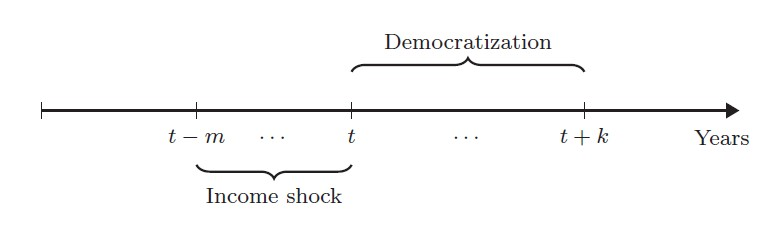
\includegraphics{img/lag.jpg}
	    \caption{Lagged effect}
	    \label{fig:lag}
	\end{figure}
	
    \noindent Note that I use either lagged dependent variable or lagged rolling average of the dependent variable (with 3 or 5 years step). I consider a lagged effect of an income shock on the political regime (or regime change) for several reasons. First, I suppose that it might require some relatively short window of time after the income shock to lead to the regime change, and it may require some time for the democratic quality institutions to change. Second, I am interested in the robust major changes in the democratic quality (or persistent low democratic quality) which is better measured by the average democratic quality score over a certain window of time rather than a single-year observation. Third, indexes might reflect changes in the quality of the democratic institutions with a certain lag. Finally, lagged dependent variable is the way to partially address the autocorrelation issue.
    \\
        \begin{figure}[ht]
        \centering
    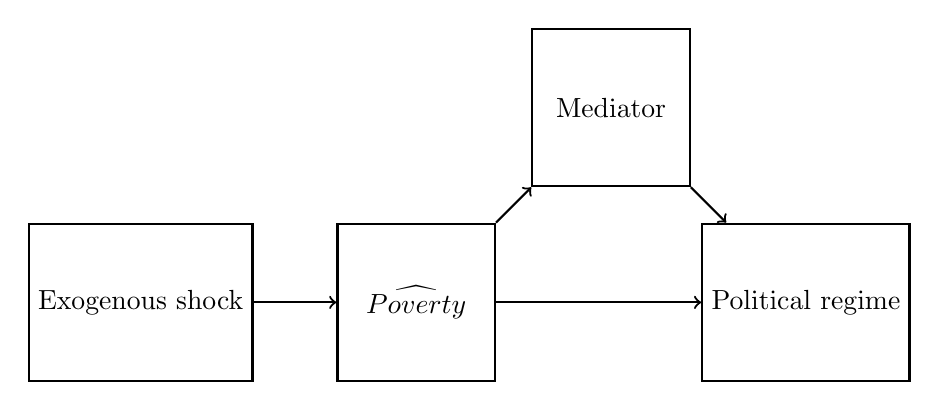
\begin{tikzpicture}[node distance={35mm}, thick, main/.style = {draw, rectangle}]
\node[main,minimum size=2cm] (1) {Exogenous shock}; 
\node[main,minimum size=2cm] (2) [right of=1] {$\widehat{Poverty}$}; 
\node[main,minimum size=2cm] (3) [above right of=2] {Mediator}; 
\node[main,minimum size=2cm] (4) [below right of=3] {Political regime}; 
\draw[->] (1) -- (2);
\draw[->] (2) -- (3);
\draw[->] (2) -- (4);
\draw[->] (3) -- (4);
\end{tikzpicture}
        \caption{Mediation analysis scheme}
        \label{fig:mediation}
    \end{figure}
    
    \noindent Last, to test the mechanisms of the relationship between poverty and political regime I use the mediation analysis. I start with the auxiliary regression to estimate the exogenous for the political regime variation in poverty:
    \begin{subequations}\label{eq:mediate}
    \begin{equation}
        p_{i,t} = \gamma s_{i,t-m|m\in\{0,3\}} + \sigma w_{i,t}+\mu_i+\tau_t +\varepsilon_{i,t}
        %\tag{\ref{eq:2sls}}
    \end{equation}
    \noindent With the fitted values of poverty $\hat p_{i,t}$ used as a non-binary treatment variable in the causal mediation analysis \parencite{mediation, mediation2}. The following equations estimate the total effect of the instrumentalized poverty on the regime:
    \begin{equation}
        d_{i, t+k|k\in\{1,5\}} = \beta_1 \hat p_{i,t} + \sigma w_{i,t}+\mu_i+\tau_t +\varepsilon_{i,t}
    \end{equation}
    \noindent The effect of the instrumentalized poverty on the mediator:
     \begin{equation}
        m_{i, t} = \beta_m \hat p_{i,t} + \sigma_m w_{i,t}+\mu_i+\tau_t +\varepsilon_{i,t}
    \end{equation}
    \noindent And the joint effect of the mediator and the treatment on the political regime:
     \begin{equation}
        d_{i, t+k|k\in\{1,5\}} = \beta_2 \hat p_{i,t} + \varphi m_{i,t} + \gamma [\hat p_{i,t} \cdot m_{i,t}] + \sigma w_{i,t}+\mu_i+\tau_t +\varepsilon_{i,t}
    \end{equation}
    \end{subequations}
    
    \noindent With the three regressions above used to decompose the total unit treatment effect into the causal mediation effect and the direct effect.
    
    

	\subsection{Data Description}

        \begin{table}[!htbp] \centering 
  \caption{Descriptive statistics} 
  \label{descr} 
  \resizebox{\textwidth}{!}{
\begin{tabular}{@{\extracolsep{5pt}}lccccccc} 
\\[-1.8ex]\hline 
\hline \\[-1.8ex] 
Statistic & \multicolumn{1}{c}{N} & \multicolumn{1}{c}{Mean} & \multicolumn{1}{c}{St. Dev.} & \multicolumn{1}{c}{Min} & \multicolumn{1}{c}{Pctl(25)} & \multicolumn{1}{c}{Pctl(75)} & \multicolumn{1}{c}{Max} \\ 
\hline \\[-1.8ex] 
Population under \$1.9 poverty line & 1,685 & 10.458 & 17.780 & 0.000 & 0.300 & 11.800 & 94.100 \\ 
Population under \$3.2 poverty line & 1,685 & 19.995 & 25.991 & 0.000 & 0.700 & 30.500 & 98.500 \\ 
Population under \$5.5 poverty line & 1,685 & 33.135 & 32.469 & 0.000 & 2.200 & 57.600 & 100.000 \\ 
Poverty gap under \$1.9 poverty line & 1,685 & 4.040 & 7.926 & 0.000 & 0.100 & 3.900 & 63.600 \\ 
Poverty gap under \$3.2 poverty line & 1,685 & 8.636 & 13.440 & 0.000 & 0.300 & 10.900 & 77.100 \\ 
Poverty gap under \$5.5 poverty line & 1,685 & 16.289 & 19.791 & 0.000 & 0.900 & 25.000 & 100.000 \\ 
PolityIV & 8,710 & 0.980 & 7.408 & $-$10.000 & $-$7.000 & 8.000 & 10.000 \\ FH score & 7,547 & 1.966 & 0.816 & 1.000 & 1.000 & 3.000 & 3.000 \\ 
PCA regime & 7,068 & 0.557 & 0.358 & 0.000 & 0.160 & 0.920 & 1.000 \\ 
Authoritarian breakdown & 3,808 & 0.047 & 0.212 & 0.000 & 0.000 & 0.000 & 1.000 \\ 
GDP pc (PPP) & 5,585 & 14,836.280 & 18,451.890 & 285.586 & 2,695.894 & 20,235.200 & 154,095.700 \\ 
GDP growth & 9,469 & 3.831 & 6.192 & $-$64.047 & 1.412 & 6.308 & 149.973 \\ 
Gini market & 5,594 & 45.552 & 6.815 & 21.800 & 41.325 & 49.400 & 72.500 \\ 
Mean years of schooling & 8,959 & 6.175 & 3.288 & 0.040 & 3.400 & 8.700 & 14.100 \\ 
Regime change & 8,805 & 0.014 & 0.118 & 0.000 & 0.000 & 0.000 & 1.000 \\ 
DD (democracy-dictatorship) & 8,208 & 0.455 & 0.498 & 0.000 & 0.000 & 1.000 & 1.000 \\ 
State capacity & 7,012 & $-$0.006 & 1.007 & $-$3.512 & $-$0.779 & 0.662 & 2.862 \\ 
Agriculture employment & 5,580 & 29.520 & 24.310 & 0.059 & 7.405 & 46.887 & 92.303 \\ 
Urban population share & 11,955 & 48.882 & 24.532 & 2.080 & 28.585 & 68.400 & 100.000 \\ 
Participation & 9,898 & 0.387 & 0.209 & 0.015 & 0.195 & 0.575 & 0.897 \\ 
\hline \\[-1.8ex] 
\end{tabular} 
}
\end{table}

	
	
	\noindent I construct an unbalanced time-series cross-sectional dataset for 170 unique country entries from 1960 to 2020 with appropriate data fullness after 1990. This sample restriction as well as the relative lack of data on the developing economies is the main limitation of the paper. Descriptive statistics are in Table \ref{descr}. As the main explanatory variable, I utilize the Poverty headcount ratio at a certain poverty line (\$1.9, \$3.2, \$5.5) a day (2011 PPP) (in the percentage of the total population of the country) from the World Development Indicators by  \cite{worldbank}. The poverty headcount ratio at a certain poverty line a day is the percentage of the population living on less than \$1.90 (\$3.2 or \$5.5) a day at 2011 international prices. I choose in favor of these estimates and not other indexes which measure poverty as a function of aggregate nationwide income statistics because it suits my theoretical framework which studies the role of a concrete group of people in poverty. Apart from that I also include the poverty gap index (for all three international poverty lines). The poverty gap is the mean shortfall from the poverty line divided by the value of the certain poverty line itself. In other words, it is the share of the poverty line that the poor people are missing, on average, in order to escape poverty.
    \\\\
	\noindent I make use of a variety of democratic quality measurements. Specifically, I utilize composite PolityIV combined score \parencite{polity}, which ranges all political regimes from -10 (institutionalized autocracy) to 10 (full institutionalized liberal democracy) with values around 0 representing the so-called anocracy. Apart from that, I create an artificial indicator based on principal components of PolityIV continuous index as well as ordinal measures of the political regime from the Varieties of Democracy project \parencite{VDemV10} and Freedom House estimate \parencite{freedomhouse}. This PCA index isolates and extracts the common variation among all three measures and combines them into a single variable that can be interpreted as democratic quality. Afterward, the PCA estimate is ranged from 0 to 1. This approach was suggested by Voigt \parencite{voigt_2013}. Finally, I construct the binary DD (democracy-dictatorship) estimate following the \parencite{democracy_growth} with the country code as a democracy if it meets the following conditions: positive PolityIV score and "free" or "partly free" score Freedom House estimate. I also include several regime changes and democratic transitions estimates: regime change from the PolityIV revised combined score where -88 states for the <<transitions>> \parencite{polity} and the data on the authoritarian breakdowns from \parencite{geddesdata}.
	\\\\
    I also include several income shock estimates. To begin with, I use the data on the systemic and banking economic crises from the \cite{bfft}. However, the concern is whether these shocks are exogenous for the government. Thus, I also utilize the binary income shocks indicator created by \cite{sjoe}. They measure major income fluctuations by a negative cyclical variation that is larger than or equal to 5 percent relative to the income trend (with a time window of three years). They decompose per capita income into the trend and the cyclical component by the HP filter, which means that the decomposition includes a certain level of randomness and can not be fully explained by the previous observations which are useful for the exogenous shocks instrument. This measure is exogenous for the following reasons: first, its randomness makes it independent of the regime's policies, second, major income fluctuations which reduce income by 5 percent occur in low- and median-income countries, which are not able to manipulate the world market.
    \\\\
    Finally, I use the branch of control variables to model the social and economic conditions of a society. Namely, I use the market (pre-tax, pre-transfer) Gini index from the Standardized World Income Inequality Database \parencite{swiid}; several more indicators from WDI: total population size, GDP per capita (PPP) and GDP growth, mean years of schooling, agriculture employment and agriculture GDP \parencite{worldbank}; finally, I use the UN population division data on the proportion of the population living in the cities \parencite{un_urb} and state capacity index from the Fragile State Indicators \parencite{state_capacity}. Last, I include several political participation indexes from the Varieties of democracy dataset \parencite{VDemV10}, specifically, I use the Participatory component index which measures both electoral and non-electoral participation of the citizens. 

	
	
	\section{Results}
	
	\subsection{Poverty and Political regimes}
	
\begin{table}[!htbp] \centering 
  \caption{Poverty and political regimes} 
  \label{plm2sls} 
  \resizebox{\textwidth}{!}{
\begin{tabular}{@{\extracolsep{5pt}}lcccc} 
\\[-1.8ex]\hline 
\hline \\[-1.8ex] 
 & \multicolumn{4}{c}{\textit{Dependent variable:}} \\ 
\cline{2-5} 
\\[-1.8ex] & \multicolumn{2}{c}{PolityIV (lag)} & \multicolumn{2}{c}{PolityIV ra 3} \\ 
\\[-1.8ex] & (1) & (2) & (3) & (4)\\ 
\hline \\[-1.8ex] 
 Population under \$1.9 poverty line & $-$0.070$^{**}$ &  & $-$0.076$^{**}$ &  \\ 
  & (0.032) &  & (0.034) &  \\ 
  & & & & \\ 
 Population under \$1.9 poverty line (IV) &  & $-$0.055$^{**}$ &  & $-$0.054$^{**}$ \\ 
  &  & (0.027) &  & (0.026) \\ 
  & & & & \\ 
 Mean years of schooling & $-$0.005 & $-$0.011 & 0.006 & $-$0.040 \\ 
  & (0.288) & (0.351) & (0.295) & (0.353) \\ 
  & & & & \\ 
 Log of GDP pc (PPP) & $-$0.922 & $-$1.226$^{*}$ & $-$1.060 & $-$1.190$^{*}$ \\ 
  & (0.682) & (0.651) & (0.666) & (0.648) \\ 
  & & & & \\ 
 Gini market & 0.056 & 0.004 & 0.061 & 0.016 \\ 
  & (0.062) & (0.055) & (0.064) & (0.057) \\ 
  & & & & \\ 
     \hline \\[-1.8ex] 
 \textit{Fixed effects}:\\
Country & Yes & Yes & Yes & Yes\\
Year & Yes & Yes & Yes & Yes\\
\hline \\[-1.8ex] 
Observations & 1,389 & 1,176 & 1,326 & 1,176 \\ 
R$^{2}$ & 0.048 & 0.009 & 0.065 & 0.009 \\ 
Adjusted R$^{2}$ & $-$0.082 & $-$0.146 & $-$0.069 & $-$0.146 \\ 
F Statistic & 15.329$^{***}_{(df = 4; 1221)}$ & 2.389$^{**}_{(df = 4; 1016)}$ & 20.131$^{***}_{(df = 4; 1159)}$ & 2.427$^{**}_{(df = 4; 1016)}$ \\ 
\hline 
\hline \\[-1.8ex] 
\footnotesize{\textit{Heteroskedasticity-robust standard-errors}}   & \multicolumn{4}{r}{$^{*}$p$<$0.1; $^{**}$p$<$0.05; $^{***}$p$<$0.01} \\ 
\end{tabular} 
}
\end{table}
	
	
	
	\noindent This section presents the results for the Models \eqref{plm}, \eqref{eq:2sls} estimating whether poverty is associated with less democratic political regimes. This preliminary analysis indicates, that higher rates of poverty are associated with the less democratic political regimes for various poverty estimates. The effect is statistically significant and robust, as the models (1) in (3) in Table \ref{plm2sls} show, and holds both for the point regime estimate and for the 3-year rolling average measure of the political regime. Figure \ref{fig:plm} presents the predicted values for both point and 3-year moving average estimate for PolityIV.
	\\
	
		\begin{figure}[!ht]
	    \centering
	    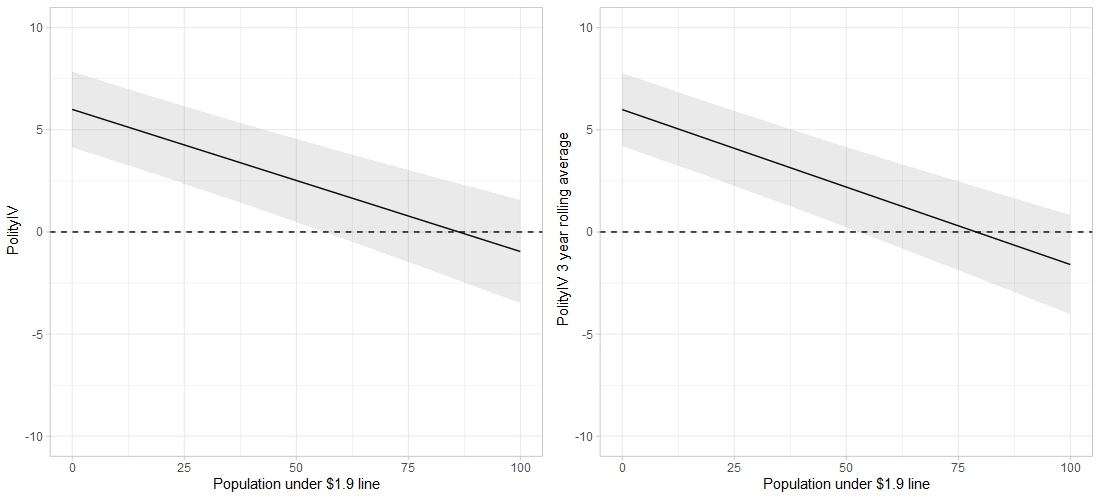
\includegraphics[width=\textwidth]{img/plm.jpeg}
	    \caption{Predicted values of PolityIV}
	    \label{fig:plm}
	\end{figure}

	
	\noindent The next models (2) and (4) in Table \ref{plm2sls} present the causal effect of instrumentalized (using exogenous negative income shocks) poverty measure. Both the direction and the significance of the effect hold for either point regime estimate and the rolling average. Predicted values of PolityIV score are in the Figure \ref{fig:iv}. The latter indicates that the effect of poverty on the regime is lasting and poverty actually does persist non-democratic rule.
	

	
	
	\subsection{Poverty and Authoritarian Survival}
	
	\begin{table}[!htbp] \centering 
  \caption{Authoritarian regimes breakdowns, LPM} 
  \label{gwffaillpm} 
  \resizebox{\textwidth}{!}{
\begin{tabular}{@{\extracolsep{5pt}}lcccccc} 
\\[-1.8ex]\hline 
\hline \\[-1.8ex] 
 & \multicolumn{6}{c}{\textit{Dependent variable:}} \\ 
\cline{2-7} 
\\[-1.8ex] & \multicolumn{6}{c}{Authoritarian regime breakdown} \\ 
\\[-1.8ex] & (1) & (2) & (3) & (4) & (5) & (6)\\ 
\hline \\[-1.8ex] 
 Population under \$1.9 poverty line & $-$0.006$^{***}$ &  &  &  &  &  \\ 
  & (0.002) &  &  &  &  &  \\ 
  & & & & & & \\ 
 Population under \$3.2 poverty line &  & $-$0.004$^{***}$ &  &  &  &  \\ 
  &  & (0.001) &  &  &  &  \\ 
  & & & & & & \\ 
 Population under \$5.5 poverty line &  &  & $-$0.001 &  &  &  \\ 
  &  &  & (0.001) &  &  &  \\ 
  & & & & & & \\ 
 Poverty gap under \$1.9 poverty line &  &  &  & $-$0.010$^{**}$ &  &  \\ 
  &  &  &  & (0.004) &  &  \\ 
  & & & & & & \\ 
 Poverty gap under \$3.2 poverty line &  &  &  &  & $-$0.008$^{***}$ &  \\ 
  &  &  &  &  & (0.003) &  \\ 
  & & & & & & \\ 
 Poverty gap under \$5.5 poverty line &  &  &  &  &  & $-$0.006$^{***}$ \\ 
  &  &  &  &  &  & (0.002) \\ 
  & & & & & & \\ 
  Mean years of schooling & 0.019 & 0.013 & 0.006 & 0.018 & 0.018 & 0.011 \\ 
  & (0.028) & (0.026) & (0.026) & (0.026) & (0.027) & (0.026) \\ 
  & & & & & & \\ 
 Log of GDP pc (PPP) & $-$0.022 & $-$0.060 & $-$0.021 & $-$0.001 & $-$0.036 & $-$0.082 \\ 
  & (0.071) & (0.075) & (0.072) & (0.072) & (0.075) & (0.076) \\ 
  & & & & & & \\ 
 Gini market & $-$0.025$^{***}$ & $-$0.017$^{*}$ & $-$0.015 & $-$0.021$^{**}$ & $-$0.021$^{**}$ & $-$0.015$^{*}$ \\ 
  & (0.010) & (0.009) & (0.010) & (0.008) & (0.009) & (0.009) \\ 
  & & & & & & \\ 
 \hline \\[-1.8ex] 
 \textit{Fixed effects}:\\
Country & Yes & Yes & Yes & Yes & Yes & Yes\\
Year & Yes & Yes & Yes & Yes & Yes & Yes\\
\hline \\[-1.8ex] 
Observations & 219 & 219 & 219 & 219 & 219 & 219 \\ 
R$^{2}$ & 0.069 & 0.044 & 0.014 & 0.053 & 0.063 & 0.050 \\ 
Adjusted R$^{2}$ & $-$0.439 & $-$0.478 & $-$0.524 & $-$0.465 & $-$0.449 & $-$0.469 \\ 
F Statistic (df = 4; 141) & 2.629$^{**}$ & 1.636 & 0.512 & 1.954 & 2.372$^{*}$ & 1.851 \\ 
\hline 
\hline \\[-1.8ex] 
\footnotesize{\textit{Heteroskedasticity-robust standard-errors in parethneses}} & \multicolumn{6}{r}{$^{*}$p$<$0.1; $^{**}$p$<$0.05; $^{***}$p$<$0.01} \\ 
\end{tabular} 
}
\end{table} 
 
	
	
	\noindent The Table \ref{gwffaillpm} presents the results for the linear probability models with the authoritarian regime breakdowns measured by \cite{geddesdata} as a binary response variable and different poverty estimates as predictors\footnote{Note that these models are estimated only on the subsample of the political regimes classified as authoritarian in the dataset by \cite{geddesdata}} corresponding to the Model \eqref{lpm}. The coefficient before most poverty estimates is negative and statistically significant at a 0.01 significance level. In other words, poverty rates significantly decrease the probability of authoritarian breakdown.
	The exception is the proportion of the population under the \$5.5 daily income line, however, it might be since, especially in the developing countries in the 20th century corresponds not to the poorest part of the population but rather to the low-middle class. Nonetheless, the coefficient remains negative yet insignificant.
	\\
    \begin{figure}[!ht]
        \centering
        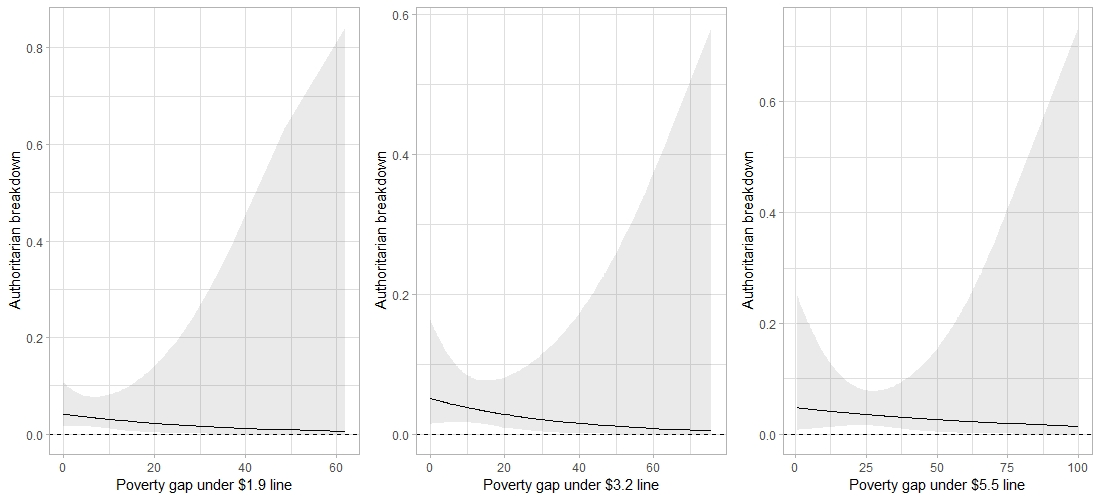
\includegraphics[width=\textwidth]{img/fails.jpeg}
        \caption{Predicted probabilities of authoritarian breakdown}
        \label{fig:fails}
    \end{figure}
    
      \begin{table}[!htbp] \centering 
  \caption{Authoritarian regimes breakdowns, conditional logit} 
  \label{gwffaillogit} 
\begin{tabular}{@{\extracolsep{5pt}}lccc} 
\\[-1.8ex]\hline 
\hline \\[-1.8ex] 
 & \multicolumn{3}{c}{\textit{Dependent variable:}} \\ 
\cline{2-4} 
\\[-1.8ex] & \multicolumn{3}{c}{Authoritarian regime breakdown} \\ 
\\[-1.8ex] & (1) & (2) & (3)\\ 
\hline \\[-1.8ex] 
 Population under \$1.9 poverty line & $-$0.096$^{**}$ &  &  \\ 
  & (0.070) &  &  \\ 
  & & & \\ 
 Population under \$3.2 poverty line &  & $-$0.073$^{*}$ &  \\ 
  &  & (0.060) &  \\ 
  & & & \\ 
 Population under \$5.5 poverty line &  &  & $-$0.036 \\ 
  &  &  & (0.072) \\ 
  & & & \\ 
  Mean years of schooling & 0.415 & 0.578 & 0.748 \\ 
  & (0.973) & (0.998) & (1.007) \\ 
  & & & \\ 
 Log of GDP pc (PPP) & $-$1.427 & $-$2.496 & $-$3.547 \\ 
  & (3.275) & (3.596) & (3.995) \\ 
  & & & \\ 
 Gini market & $-$0.524 & $-$0.321 & $-$0.239 \\ 
  & (0.745) & (0.823) & (0.835) \\ 
  & & & \\ 
  \hline \\[-1.8ex] 
 \textit{Fixed effects}:\\
Country & Yes & Yes & Yes\\
Year & No & No & No \\
\hline \\[-1.8ex] 
Observations & 219 & 219 & 219 \\ 
R$^{2}$ & 0.019 & 0.016 & 0.008 \\ 
Max. Possible R$^{2}$ & 0.115 & 0.115 & 0.115 \\ 
Log Likelihood & $-$11.289 & $-$11.635 & $-$12.478 \\ 
Wald Test (df = 4) & 7.540 & 6.110 & 2.780 \\ 
LR Test (df = 4) & 4.141 & 3.447 & 1.763 \\ 
Score (Logrank) Test (df = 4) & 3.930 & 3.176 & 1.620 \\ 
\hline 
\hline \\[-1.8ex] 
\footnotesize{\textit{Robust standard-errors in parentheses}}  & \multicolumn{3}{r}{$^{*}$p$<$0.1; $^{**}$p$<$0.05; $^{***}$p$<$0.01} \\ 
\end{tabular} 
\end{table}

    	
    \noindent The next Table \ref{gwffaillogit} corresponds to the Model \eqref{logitfail} and estimates the same specification as the Table \ref{gwffaillpm} but using the logistic regression and excluding time fixed effects as the sample size is insufficient for the model to converge. The result obtained in the linear probability model holds. Poverty rates are associated with the statistically significant negative effect on the probability of the authoritarian breakdown, with the significance decreasing for the higher poverty lines.
    
	
	\subsection{Poverty, Income Shocks and Democratization}
	
	\noindent Here I test the impact of negative income shocks on the quality of the democratic institutions and democratization conditional on poverty. First, I make the difference in PolityIV score, use two different poverty estimates and interact with negative exogenous income shock which is corresponding to the Model \eqref{democ}. The results\footnote{Note that additional controls are included in the models but were not reported in the regression summary tables for the matter of simplicity} are presented in Table \ref{nshock:democ} and the Margin effects in the Figure \ref{fig:medemoc}.
	\\
	\begin{table}[!htbp] \centering 
  \caption{Negative income shocks and democratization} 
  \label{nshock:democ} 
  \resizebox{\textwidth}{!}{
\begin{tabular}{@{\extracolsep{5pt}}lcc} 
\\[-1.8ex]\hline 
\hline \\[-1.8ex] 
 & \multicolumn{2}{c}{\textit{Dependent variable:}} \\ 
\cline{2-3} 
\\[-1.8ex] & \multicolumn{2}{c}{$\Delta$ Polity IV (lagged)} \\ 
\\[-1.8ex] & (1) & (2)\\ 
\hline \\[-1.8ex] 
Population under \$1.9 poverty line & $-$0.018$^{**}$ &  \\ 
  & (0.009) &  \\ 
  & & \\ 
 Poverty gap under \$1.9 poverty line &  & $-$0.037$^{**}$ \\ 
  &  & (0.017) \\ 
  & & \\ 
 PolityIV & $-$0.160$^{***}$ & $-$0.159$^{***}$ \\ 
  & (0.029) & (0.030) \\ 
  & & \\ 
  Negative shock & $-$0.074 & $-$0.076 \\ 
  & (0.072) & (0.076) \\ 
  & & \\ 
  Population under \$1.9 line:Negative shock & 0.009$^{**}$ &  \\ 
  & (0.004) &  \\ 
  & & \\ 
 Poverty gap under \$1.9 line:Negative shock &  & 0.024$^{**}$ \\ 
  &  & (0.010) \\ 
  & & \\ 
  \hline \\[-1.8ex] 
\textit{Fixed effects}:\\
Country & Yes & Yes\\
Year & Yes & Yes\\
\hline \\[-1.8ex] 
Observations & 1,358 & 1,358 \\ 
R$^{2}$ & 0.098 & 0.100 \\ 
Adjusted R$^{2}$ & $-$0.047 & $-$0.044 \\ 
F Statistic (df = 4; 1169) & 31.868$^{***}$ & 32.605$^{***}$ \\ 
\hline 
\hline \\[-1.8ex] 
\footnotesize{\textit{Heteroskedasticity-robust standard-errors}} & \multicolumn{2}{r}{$^{*}$p$<$0.1; $^{**}$p$<$0.05; $^{***}$p$<$0.01} \\ 
\end{tabular} 
}
\end{table} 
	
		\begin{figure}[ht]
	    \centering
	    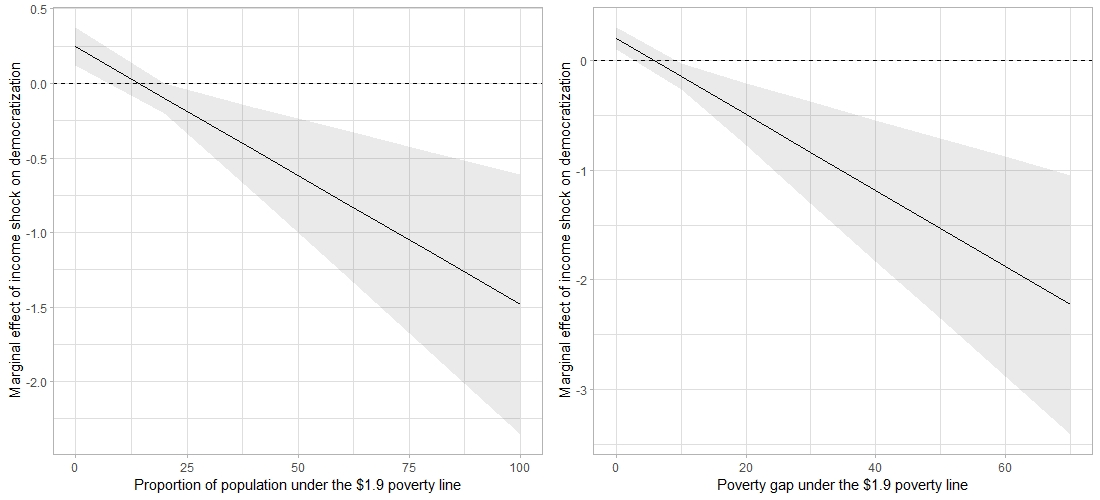
\includegraphics[width=\textwidth]{img/medemoc.jpeg}
	    \caption{Margin effect of negative income shock on democratization}
	    \label{fig:medemoc}
	\end{figure}
	
	\noindent Here both the proportion of the population under \$1.9 poverty line and the poverty gap index themselves have statistically significant (at p<0.05 significance level) negative coefficient. As well, note that the interaction effects between the poverty estimates and the negative exogenous income shock have a statistically significant positive effect on the difference in the quality of the democratic institutions. The margin effects of the exogenous negative income shocks (see Figure \ref{fig:medemoc}) tell the full story: the effect is positive and statistically significant\footnote{As the confidence intervals do not cover zero} at the low levels of poverty rates -- however, note that most states are concentrated around almost zero poverty levels (see Figure \ref{fig:povhists} in the Appendix) --  and becomes negative significant for the higher levels of poverty, nonetheless the confidence intervals become wider.
	\\
	

	
	\begin{table}[!htbp] \centering 
  \caption{Negative income shocks and (lagged) democratic quality} 
  \label{nshock:dem} 
  \resizebox{\textwidth}{!}{
\begin{tabular}{@{\extracolsep{5pt}}lccc} 
\\[-1.8ex]\hline 
\hline \\[-1.8ex] 
 & \multicolumn{3}{c}{\textit{Dependent variable:}} \\ 
\cline{2-4} 
\\[-1.8ex] & Polity IV & Polity ra 3 & Polity ra 5 \\ 
\\[-1.8ex] & (1) & (2) & (3)\\ 
\hline \\[-1.8ex] 
 Population under \$1.9 poverty line & $-$0.053 & $-$0.059$^{*}$ & $-$0.057$^{*}$ \\ 
  & (0.034) & (0.033) & (0.033) \\ 
  & & & \\ 
 Negative shock & 0.167 & 0.199 & 0.172 \\ 
  & (0.239) & (0.225) & (0.222) \\ 
  & & & \\ 
 Population under \$1.9 line:Negative shock & 0.002 & 0.001 & 0.004 \\ 
  & (0.016) & (0.015) & (0.013) \\ 
  & & & \\ 
  \hline \\[-1.8ex] 
\textit{Fixed effects}:\\
Country & Yes & Yes & Yes\\
Year & Yes & Yes & Yes\\
\hline \\[-1.8ex] 
Observations & 1,359 & 1,358 & 1,358 \\ 
R$^{2}$ & 0.025 & 0.036 & 0.039 \\ 
Adjusted R$^{2}$ & $-$0.131 & $-$0.118 & $-$0.115 \\ 
F Statistic (df = 3; 1170) & 9.954$^{***}$ & 14.472$^{***}$ & 15.856$^{***}$ \\ 
\hline 
\hline \\[-1.8ex] 
\footnotesize{\textit{Heteroskedasticity-robust standard-errors}} & \multicolumn{3}{r}{$^{*}$p$<$0.1; $^{**}$p$<$0.05; $^{***}$p$<$0.01} \\ 
\end{tabular} 
}
\end{table}

		\begin{figure}[ht]
	    \centering
	    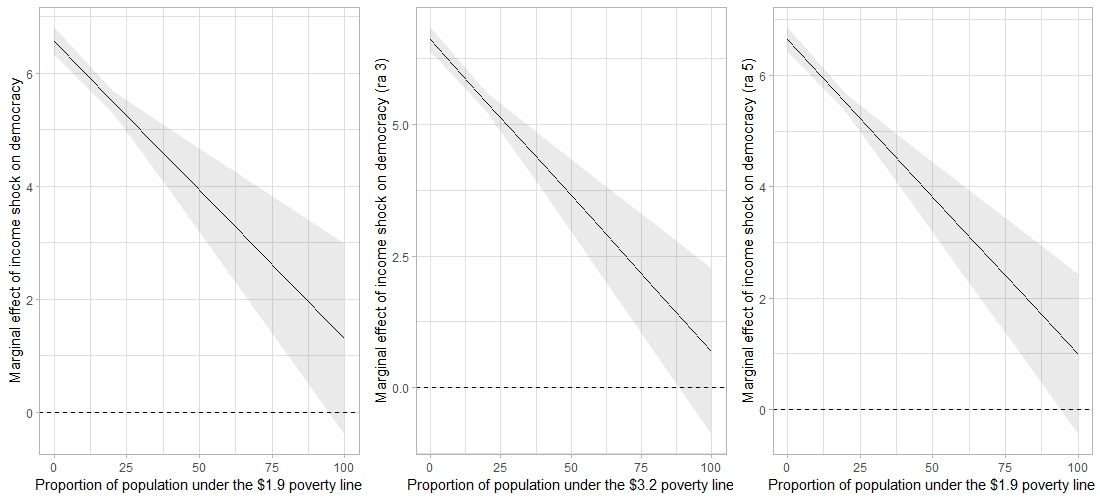
\includegraphics[width=\textwidth]{img/medem.jpeg}
	    \caption{Margin effect of negative income shock on democratic quality}
	    \label{fig:medem}
	\end{figure}
	
	\noindent The Table \ref{nshock:dem} shows the effect of poverty in presence of an income shock, corresponding to the Model \eqref{dem} and the Figure \ref{fig:medem} shows margin effects. Response variables are either a simple lagged PolityIV score or lagged rolling average of PolityIV score (with 3 or 5-year step). The coefficient before interaction terms are statistically insignificant which means that income shocks in states with a large share of the population under the poverty line do not impact the quality of democratic institutions. And as the margin effect is decreasing for all three response variables the result is that higher poverty rates make the effect insignificant while states with a lower proportion of the population in poverty income shocks have significant positive income on democratic quality.
	\\
    
    \noindent Note, that these findings stand in line with the findings from the previous subsection, as the coefficient before poverty measure itself is negative (and for some models statistically significant), which implies that in absence of an income shock (i.e. if the interaction term nullifies) higher poverty rates have a negative effect on both democratization and the quality of democratic institutions themselves.
	\\\\
	\noindent To sum up the empiric part of the paper: (a) states with higher levels of poverty are significantly less democratic, moreover, poverty causes lower democratic institutions quality (b) poverty statistically significant decreases the probability of the authoritarian breakdown (c)  however, the interaction between the poverty rates and the exogenous negative income shocks does cause the short-term democratization, (d) nonetheless, it does not have a positive impact on the long-term quality of the democratic institutions.
	
	\section{Robustness}
    
    First, I check for the robustness of the results by using different political regimes and poverty measures within the same identification strategy. Precisely, I utilize the PCA regime measure, described above and test the results with higher poverty lines. However, it is crucial to mention that different poverty lines reflect a bit different social groups, as in the developing countries the difference between \$1.9 and \$5.5 daily consumption can be significant. This means, that possible difference in results between these poverty lines does not necessarily imply that the model is not robust. Regression summary tables for all combinations of response and independent variables as well as the estimation methods are reported in the Appendix. The direction and the significance of the effect hold for all the models.
    \\
    
   \begin{table}[!htbp] \centering 
  \caption{Regime change, LPM} 
  \label{lpmrc} 
  %\resizebox{\textwidth}{!}{
\begin{tabular}{@{\extracolsep{5pt}}lccc} 
\\[-1.8ex]\hline 
\hline \\[-1.8ex] 
 & \multicolumn{3}{c}{\textit{Dependent variable:}} \\ 
\cline{2-4} 
\\[-1.8ex] & \multicolumn{3}{c}{Regime change (lagged)} \\ 
\\[-1.8ex] & (1) & (2) & (3)\\ 
\hline \\[-1.8ex] 
 Population under \$1.9 poverty line & $-$0.001$^{***}$ &  &  \\ 
  & (0.0003) &  &  \\ 
  & & & \\ 
 Population under \$3.2 poverty line &  & $-$0.001$^{***}$ &  \\ 
  &  & (0.0002) &  \\ 
  & & & \\ 
 Population under \$5.5 poverty line &  &  & $-$0.0005$^{**}$ \\ 
  &  &  & (0.0002) \\ 
  & & & \\ 
 DD & $-$0.047$^{***}$ & $-$0.054$^{***}$ & $-$0.044$^{***}$ \\ 
  & (0.010) & (0.012) & (0.014) \\ 
  & & & \\ 
 Population under \$1.9 line:DD & 0.001$^{***}$ &  &  \\ 
  & (0.0003) &  &  \\ 
  & & & \\ 
 Population under \$3.2 line:DD &  & 0.001$^{***}$ &  \\ 
  &  & (0.0002) &  \\ 
  & & & \\ 
 Population under \$5.5 line:DD &  &  & 0.0003 \\ 
  &  &  & (0.0002) \\ 
  & & & \\ 
    \hline \\[-1.8ex] 
 \textit{Fixed effects}:\\
Country & Yes & Yes & Yes\\
Year & Yes & Yes & Yes \\
\hline \\[-1.8ex] 
Observations & 1,388 & 1,388 & 1,388 \\ 
R$^{2}$ & 0.019 & 0.021 & 0.012 \\ 
Adjusted R$^{2}$ & $-$0.117 & $-$0.115 & $-$0.125 \\ 
F Statistic (df = 6; 1218) & 3.983$^{***}$ & 4.398$^{***}$ & 2.556$^{**}$ \\ 
\hline 
\hline \\[-1.8ex] 
\textit{Controls included}  & \multicolumn{3}{r}{$^{*}$p$<$0.1; $^{**}$p$<$0.05; $^{***}$p$<$0.01} \\ 
\end{tabular}
%}
\end{table}
    
    \noindent Table \ref{lpmrc} shows the results for the Model \eqref{lpmchange}, testing whether the effect of poverty on the regime collapse is homogeneous for democratic and non-democratic political regimes. As the DD (democracy-dictatorship) index takes value 1 for the democratic regimes, the effects of poverty on the authoritarian breakdown are shown by the coefficient before the poverty estimate itself as for the authoritarian regimes DD measure takes value 0 thus nullifying the interaction term. So, for the non-democratic political regimes poverty sadistically significantly decreases the probability of the regime change, which supports the results obtained above in the Tables \ref{gwffaillpm} and \ref{gwffaillogit}. However, for democracies the result is different. The coefficient before the dummy variable for democracy is negative and significant. It implies that democracies, on average, face fewer regime changes. Nonetheless, the coefficient before the interaction term is positive and significant which indicates that in democracies, unlike authoritarian regimes, poverty increases the probability of regime change. It stands in line with the literature, suggesting that the economic performance is crucial for the democratic and insignificant for the authoritarian survival \parencite{hazard_rate}.
    \\\\
    \noindent Finally, I include additional controls for possible alternative explanations. I include two main groups of controls, first, for state capacity as one might suppose that poverty itself is just the consequence of the lower ability of the state to provide basic goods. Second, I control for several correlates of poverty, not included in the specifications used above. Namely, I include controls for the urban population share and the agriculture employment in the economy. The idea is that if the poor people live in the countryside and not in the cities it makes it harder for them to control the government compares to the urban population \parencite{campante1}. Regression summary tables are, again, presented in the Appendix. Both the direction and statistical significance of the effect hold, which I interpret as the sign that the discovered effect is the effect of poverty itself rather than of its correlates.   

    \section{Mechanism}
    
    \noindent Apart from that, I propose a mechanism that can explain the effect, theoretically described and empirically identified above. The basic assumption of my formal model was relatively higher costs of participating in the revolution for the citizens with low income compared to the ones with the high. The participation in the <<revolt>> in my model could be interpreted more broadly as the voluntary (on the contrary to the co-optation for prizes) participation in politics as such. Thus, I suggest the following mechanism: higher poverty rates lower voluntary democratic participation, which in turn lowers the quality of the democratic institutions. 
    \\
    
        \begin{table}[!htbp] \centering 
  \caption{Mediation analysis auxiliary regressions} 
  \label{mediate} 
  \resizebox{\textwidth}{!}{
\begin{tabular}{@{\extracolsep{5pt}}lccc} 
\\[-1.8ex]\hline 
\hline \\[-1.8ex] 
 & \multicolumn{3}{c}{\textit{Dependent variable:}} \\ 
\cline{2-4} 
\\[-1.8ex] & PolityIV & Participation & PolityIV \\ 
\\[-1.8ex] & (1) & (2) & (3)\\ 
\hline \\[-1.8ex] 
 Population under \$1.9 poverty line (IV) & $-$0.047 & $-$0.002$^{*}$ & $-$0.018 \\ 
  & (0.031) & (0.001) & (0.026) \\ 
  & & & \\ 
 Participation &  &  & 12.692$^{***}$ \\ 
  &  &  & (4.824) \\ 
  & & & \\ 
 Mean years of schooling & $-$0.048 & $-$0.005 & 0.012 \\ 
  & (0.338) & (0.011) & (0.262) \\ 
  & & & \\ 
 Log of GDP pc (PPP) & $-$0.547 & $-$0.032 & $-$0.144 \\ 
  & (0.703) & (0.037) & (0.621) \\ 
  & & & \\ 
 Gini market & 0.020 & $-$0.001 & 0.033 \\ 
  & (0.058) & (0.002) & (0.056) \\ 
  & & & \\ 
      \hline \\[-1.8ex] 
 \textit{Fixed effects}:\\
Country & Yes & Yes & Yes\\
Year & Yes & Yes & Yes \\
\hline \\[-1.8ex] 
Observations & 1,176 & 1,176 & 1,176 \\ 
R$^{2}$ & 0.003 & 0.014 & 0.146 \\ 
Adjusted R$^{2}$ & $-$0.153 & $-$0.140 & 0.011 \\ 
F Statistic & 0.841 (df = 4; 1016) & 3.714$^{***}$ (df = 4; 1016) & 34.605$^{***}$ (df = 5; 1015) \\ 
\hline 
\hline \\[-1.8ex] 
\footnotesize{\textit{Heteroskedasticity-robust standard-errors}}  & \multicolumn{3}{r}{$^{*}$p$<$0.1; $^{**}$p$<$0.05; $^{***}$p$<$0.01} \\ 
\end{tabular} 
}
\end{table} 
    
       \begin{table}[!htbp]
        \centering
        \caption{Causal mediation analysis}
        \label{mediateres}
        \resizebox{\textwidth}{!}{
        \begin{tabular}{@{\extracolsep{5pt}}lcccc} 
\\[-1.8ex]\hline 
\hline \\[-1.8ex] 
\\[-1.8ex] & Estimate & 95\% CI Lower & 95\% CI Upper & p-value \\ 
\hline \\[-1.8ex] 
  ACME & $-$0.0284  &   $-$0.0475  & $-$0.01 &  0.004$^{***}$   \\
  & & &  &\\ 
  ADE  & $-$0.0193  &    $-$0.0646   &    0.03 &   0.432 \\
  & & &  &\\ 
  Total Effect  &  $-$0.0476   &   $-$0.0994    &     0.01  & 0.074$^{*}$ \\
  & & &  &\\ 
  Prop. Mediated &   0.5672    &  -1.2828    &    2.91 &  0.078$^{*}$ \\
  & & &  &\\ 
  \hline 
\hline \\[-1.8ex] 
\footnotesize{\textit{Quasi-Bayesian Confidence Intervals}}  & \multicolumn{4}{r}{$^{*}$p$<$0.1; $^{**}$p$<$0.05; $^{***}$p$<$0.01} \\ 
        \end{tabular}
        }
    \end{table}
    
    \noindent First, I check whether the mediation effect exists, estimating the Model \eqref{eq:mediate}. Table \ref{mediate} presents the auxiliary regressions. The results for these supplementary models stand in line with the previous findings, as instrumentalized poverty has a negative effect on the quality of the democratic institutions (see Table \ref{plm2sls}). What is more important, higher poverty rates have a significant negative effect on participation (participatory component index). This means that poverty negatively affects democratic participation. Last, the result is that participation has a significant positive effect on the quality of the democratic institutions (which also stands in line with the theoretical expectations).
    \\
     \begin{figure}[httbt]
        \centering
        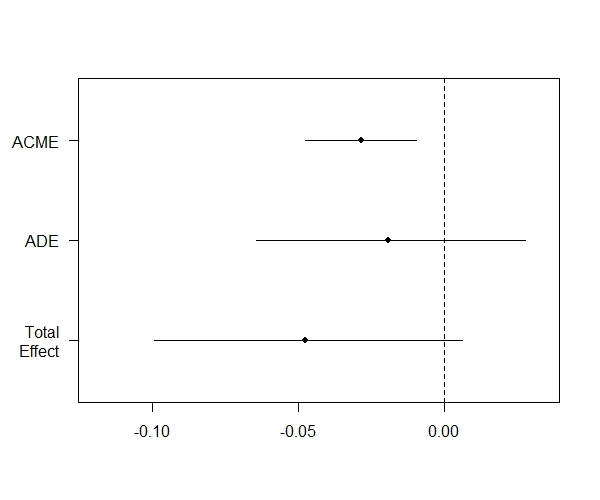
\includegraphics[width=0.75\textwidth]{img/mediation.jpeg}
        \caption{Average causal mediation, direct, and total effects}
        \label{fig:mediate}
    \end{figure}
    
    \noindent Next, I use these auxiliary models to fit the mediation analysis with the quasi-Bayesian approximation to estimate the confidence intervals. The Figure \ref{fig:mediate} and the Table \ref{mediateres} present the point estimate and the 95\% confidence interval bounds. ACME stands for the average causal mediation effect, which is the indirect effect of poverty on the political regime through participation in political processes. The plot indicates that the average causal mediation effect is negative and statistically significant as the confidence interval does not cover zero. This means that the effect of (instrumentalized) poverty rate on the democratic institutions' quality, going through the (lower) participation in politics. ADE is the average direct effect -- which is essentially the effect of (instrumentalized) poverty on the political regime with control for the mediator (see Model 3 from Table \ref{mediate}) and is negative yet insignificant. The total effect is in essence the sum of the direct and indirect (i.e. mediated) effect of poverty on the political regime. The total effect is negative and boundary statistically significant. Finally, Table \ref{mediateres} shows the proportion of the effect of poverty which goes through the mediator (i.e. the participation in politics) and equals 0.57. In other words, just over half of the effect is mediated by the lower participation in politics, which again is the boundary statistically significant. 
    
   

    
    
    %\subsection{Failed democratization}
    
    %\noindent Last, I check why the democratization in the states with the higher poverty rates is less likely to succeed. 
        
    
	
	\section{Discussion}
	
	In this section, I review and reinterpret the results of the empirical analysis in the broader context and put them in line with the theoretical framework. I will focus on some anecdotal evidence on certain cases, supporting my inference. To begin with, here are the key findings of the paper so far (a) states with higher poverty rates are significantly less democratic, moreover poverty causes lower democratic quality in long-term; (b) poverty significantly decreases the probability of the authoritarian breakdown; (c) poverty (partially) hinders the democratic window of opportunity, caused by the exogenous income shock; (d) the mechanism is significantly lower participation in politics, caused by the poverty, which reduces the quality of the democratic institutions.
	\\\\
	I would start with several examples of poor states with persistent authoritarian regimes. Laos also knows as the Lao People's Democratic Republic remains under the ruling communist party authoritarian rule since 1975 when communists won the civil war. There were no free elections with independent candidates allowed in Laos since then. Independent judiciary is absent as well as the freedom of expression and independent self-organization \parencite{laos}. At the same time, Laos remained the state with much higher poverty rates than the mean for the world, with the last reported estimate of the proportion of the population under \$1.9 poverty line equal 22.7\% in 2012 (mean value for that year was around 5.85\%). Partly, the government itself is responsible for this trend as it fails (or is not willing) to employ economic growth to overcome the social issues \parencite{laos2}. There was no mass struggle for democratization within the country, participation in politics score is also below average. As expected, for the state where the majority of the population lives for less than \$5.5 a day and is more interested to make both ends meet rather than spending time on the political struggle, facing inevitable costs. Illustratively, the government officials seem to be more afraid of the spill-over effect of democratization movement in the region, rather than the endogenous uprising \parencite{laos3}.
	\\\\
	Another illustration is contemporary Angola, the ex-Portuguese colony. The nation is poorer, with 47.6\% of the population living below the \$1.9 daily consumption poverty line in 2018, despite the wealth in natural resources. The participatory component index is three times below the world's average. Nonetheless, Angola is an example of more modern, electoral authoritarianism with a multiparty system and regular election. Still, there is little to no chance for the opposition to win such elections \parencite{angola}. The regime co-opts the poor with various social programs, such as house delivery, serving as prizes for loyalty \parencite{angola2}. This allows the government to partly control both the poor and the poverty rates, keeping the society under control. As the regime posses high gains from oil exports it can afford large co-optation programs, yet, poverty is high. All of these manipulations result in the persistent competitive authoritarian regime \parencite{oldway, newway}, which allows certain <<facade>> political activity, but restricts possible actual opposition. The strategy of the regime is to artificially lower the incentives for voluntary pro-democratic political participation, which strengthens the effect of poverty. At the same time, the elites are able to enjoy the uncontested rent from the natural resources \parencite{angola3}. In other words, these two cases show how poverty hinders the political participation of the people, thus inhibiting the struggle for democracy and how the elites and the government use various strategies to further prevent the pro-democratic movements. 
	\\
	
	\noindent Next, I move on to a couple of examples of (unsuccessful) democratization in poor states. The small country of Haiti is located on the Western half of Hispaniola island. Haiti is known as the least developed American state, in the contrast with the developed neighbor -- the Dominican Republic \parencite{haiti1, haiti2}. Haiti became the second independent American nation (after the US) in 1804, however, it had not become a democracy and faced occupation in the early XX century. History resulted in the thirty years of Duvalier family rule, which ended in 1985 \parencite{haiti3, haiti4}. Nonetheless, started democratization was delayed by several coups and the short military rule \parencite{haiti5}. Only in 1994, after the US military intervention (and during the major economic crisis, partly caused by the sanctions) the president-elect Jean-Bertrand Aristide was returned to power \parencite{haiti6}. Nevertheless, in the early 2000s, the government during Aristide's second term abused the power and committed several human rights violations, which resulted in another political crisis. Another foreign military and UN intervention helped to restore the order and stop the violence after a while, still, the state is weak and unable to implement its basic capacities \parencite{haiti7}. The left side of the Figure \ref{fig:HTIGNB} shows the PolityIV score for Haiti since 1985 and indicates several major fluctuations, which obstruct any sustainable building of a strong and capable government. At the same time, despite a quarter of the population living on less than \$1.9 poverty line, participation in politics remained just below the world average since the late 1990s (expected, for the nation with such a vivid recent political history), yet this was rarely participating in the democratic political processes. However, this example indicates that not just political participation per se matters for the quality of the democratic institutions, but the participation in the institutionalized, democratic processes. 
	\\
	\begin{figure}[ht]
	    \centering
	    \subfloat[\centering Haiti]{{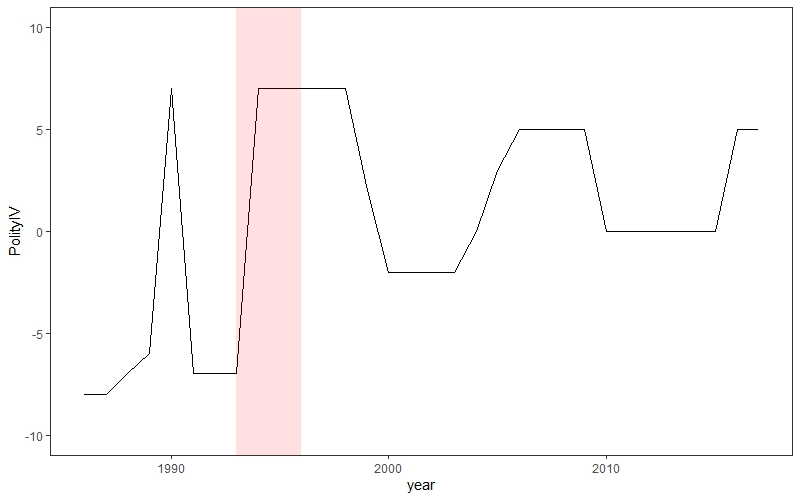
\includegraphics[width=7.1cm]{img/HTI} }}%
        \qquad
        \subfloat[\centering Guinea-Bissau]{{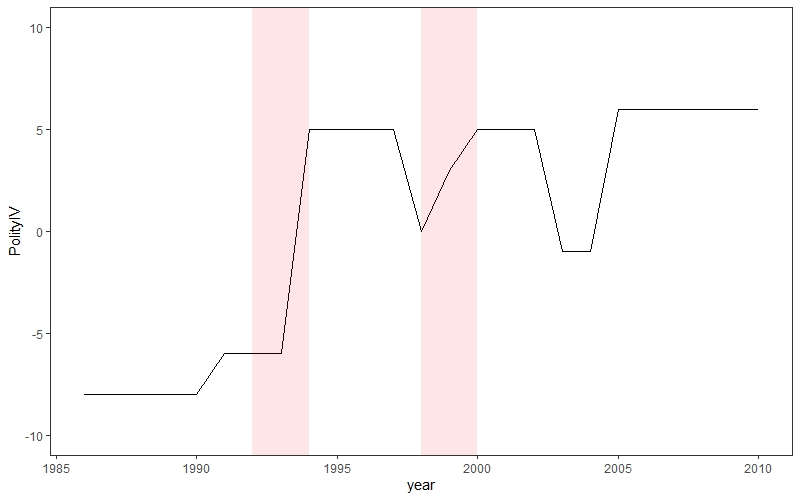
\includegraphics[width=7.1cm]{img/GNB} }}
	    \caption{Failed democratization, red filled area -- negative income shock}
	    \label{fig:HTIGNB}
	\end{figure}
	
	\noindent The last story is about the Western African state of Guinea-Bissau, another ex-Portuguese colony. In 1974 after the war and the revolution it gained independence. However, the established regime was a PGAIC (African Party for the Independence of Guinea and Cape Verde) communist dictatorship, supported by the Soviet Union and Cuba. In 1980 after the elite coup slow political democratization and economic liberalization began. New Constitution was adopted in 1989 and legalized independent political parties. First multiparty elections were held in 1994 \parencite{guinea1}. As the right side of the Figure \ref{fig:HTIGNB} illustrates, it was also the time of the major economic crisis. In 1998, during another major economic crisis, a popular, and army uprising resulted in the civil war. The president Jo{ã}o Bernardo Vieira remained in power, with the assist of the foreign military, until 1999 when the president was expelled and the new elections were held. However, the military coup happened again in 2004, with Vieira re-elected afterward. Nonetheless, the president was killed later, leading to another electoral cycle \parencite{guinea2}. Endless repetition of the military coups and elections continues. One can notice that, except for the times of the major negative income shocks, the political process was shaped by either the partisan elites or the military, while the people kept aloof. This observation, however, is expected, as more than half of the population lives on less than \$1.9 a day, and, consequently, does not participate much in politics. That is to say, Guinea-Bissau is a topical example of a nation, where poverty hindered the democratic window of opportunity, opened up by the major economic crises, as the popular uprisings did not result in the long-term struggle for the capable yet democratic state \parencite{guinea4}. It is also important to mention, that during the political fluctuations, described above, Guinea-Bissau became the first so-called 'narco-state', as the country is on the trafficking routes of the Columbian cartels and the officials (and the military) are involved and benefit, as they receive bribes, from the process \parencite{guinea3}. Although the nation does not suffer from the ruling party authoritarian regime anymore, the poverty did not allow the people to continue the struggle and apply pressure on the government, as the state was captured by the corrupted elites and the military.
	\\
	
	\noindent Last, the mechanism, discovered in this paper stands in line not only with several historical cases with the recent institutionalism studies. First, we can interpret the lower participation in democratic political processes of the poor citizens as the indicator of the <<weak>> society. In other terms, the nation with higher poverty rates is not able to apply enough pressure on the government, allowing the state to dominate. This results either in the sustainable dictatorship, which starts to restrict the society, like in China (in the XX century) or Laos. Poverty also shuts down the possible democratic window of opportunity, decreasing the possible democratization or allowing the elites to capture the state back as the poor do not apply pressure afterward. This leads to the weak, unstable, and sometimes even failed state, not able to achieve its basic goals and capacities like in Haiti or Guinea-Bissau. That is, such a nation is not powerful enough to <<shackle the Leviathan>> \parencite{corridor}. Second, the nation with the higher proportion of the population in poverty faces the exclusion of a certain group from politics \parencite{exclusion}, as was shown above. It increases the inequality and shifts the balance of power between the other groups, as the relative weight of the elites' resources increases, thus persisting the status-quo, as it happens in Angola \parencite{inst_per}.
	
	
	\section{Conclusion}
	
	\noindent In this paper I examined how does poverty sustain dictatorship. My key assumption is based upon the evidence that chronicle poverty results in biased time preferences \parencite{poverty_consequences}: the poor value current consumption much higher than the future relative to the citizens with higher income. I present a simple formal model, which is the modification of the classical public good creation game with two types of agents with different incomes. I suppose that due to the biased time preferences the poor might choose short-term benefits from co-optation to the long-term utility of the revolt, thus the higher proportion of the poor in the population reduces the probability of revolt and makes the state less democratic. However, the exogenous income shock can open the window of opportunity for the poor to overthrow the regime (as in such case they have almost literally <<nothing to lose but their chains>>).
	\\\\
	Next, I test empirically the propositions of the theoretical model. The results are that poverty is associated with the less democratic political regime, furthermore instrumentalized poverty does cause lower democratic institutions quality in the near term, poverty decreases the probability of the authoritarian breakdown, and degrades the effect of an income shock on possible democratization. I check for the possible mechanism and find that the effect of poverty is partially mediated by lower participation in politics. 
	\\\\
	Last, I provide some topical examples and show the applicability of the mechanism to explain some real-world cases of persistent stable authoritarianism in Laos and Angola, and failed democratization of Haiti and Guinea-Bissau. I adjust the proposed theoretical mechanisms, as the case of Haiti shows that the poor can participate actively in politics, yet the political process might be destructive for the nation. Thus, I suppose that participation in the institutionalized democratic political processes is the key. I also put the findings of the paper in line with the modern institutional political economy.
	\\\\
	Nonetheless, the study still faces certain limitations, namely sample restrictions as the panel poverty data of full value is available only for a relatively short amount of time. Which is worse, there is a lack of data on the poorest developing countries, which leads to a potential sample-selection bias in empirical analysis. A further, detailed study using individual-level data to verify the micro-level theoretical mechanism is required. 
	\\\\
	To sum up, this study shows how people's poverty perpetuates dictatorship. The overestimation of the short-term consumption compare to the long-term benefits by the poor (a) makes them vulnerable for the co-optation by the regime (b) reduces their ability to spend time participating in politics. This effect makes the states with higher poverty rates (1) less democratic (2) less likely, to overthrow the dictatorship (c) less likely to benefit from the democratic window of opportunity, opened up by the exogenous income shocks.
	
	
	\newpage
    \section{Appendix}
	
%	\subsection*{Proof for the Formal Model}
	
	
	
%	\subsection*{Variables Visualizations}
	
	\begin{figure}[ht]
	    \centering
	    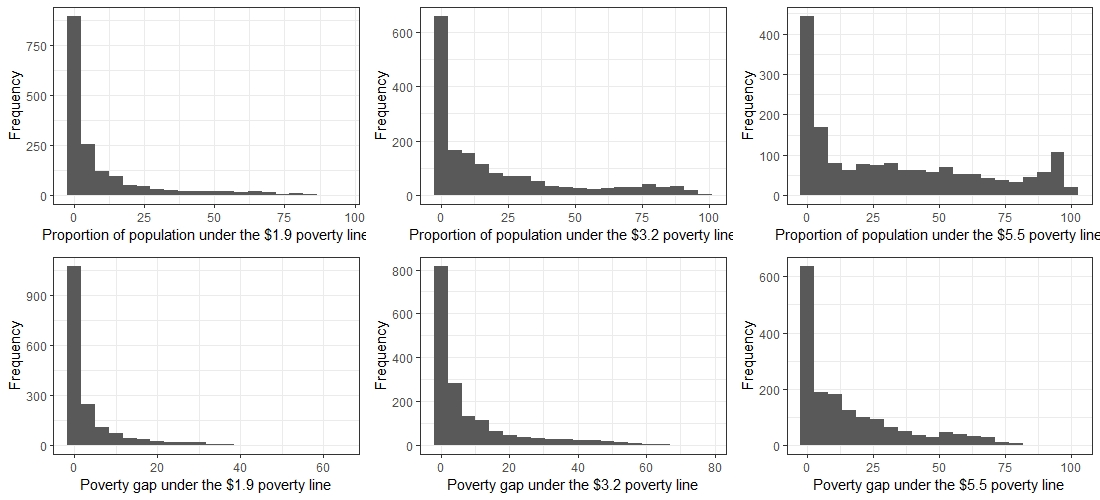
\includegraphics[width=\textwidth]{img/povhists.jpeg}
	    \caption{Poverty rates distributions}
	    \label{fig:povhists}
	\end{figure}
	
    \begin{figure}[ht]
	    \centering
	    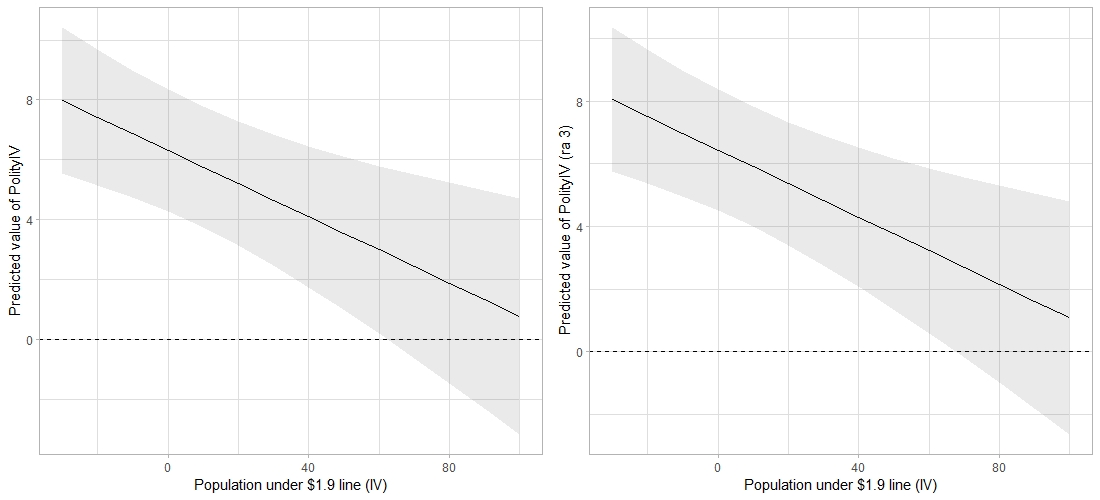
\includegraphics[width=\textwidth]{img/iv.jpeg}
	    \caption{Predicted PolityIV score, 2SLS models}
	    \label{fig:iv}
	\end{figure}
	
%	\subsection*{Regression Summary Tables}
	

\begin{table}[!htbp] \centering 
  \caption{Poverty and political regimes} 
  \label{plmm} 
  \resizebox{\textwidth}{!}{
\begin{tabular}{@{\extracolsep{5pt}}lcccc} 
\\[-1.8ex]\hline 
\hline \\[-1.8ex] 
 & \multicolumn{4}{c}{\textit{Dependent variable:}} \\ 
\cline{2-5} 
\\[-1.8ex] & \multicolumn{2}{c}{PolityIV (lag)} & \multicolumn{2}{c}{PolityIV ra 3} \\ 
\\[-1.8ex] & (1) & (2) & (3) & (4)\\ 
\hline \\[-1.8ex] 
 Population under \$1.9 poverty line & $-$0.070$^{**}$ &  & $-$0.076$^{**}$ &  \\ 
  & (0.032) &  & (0.034) &  \\ 
  & & & & \\ 
 Population under \$3.2 poverty line &  & $-$0.048$^{**}$ &  & $-$0.048$^{*}$ \\ 
  &  & (0.024) &  & (0.025) \\ 
  & & & & \\ 
 Mean years of schooling & $-$0.005 & $-$0.050 & 0.006 & $-$0.044 \\ 
  & (0.288) & (0.301) & (0.295) & (0.310) \\ 
  & & & & \\ 
 Log of GDP pc (PPP) & $-$0.922 & $-$1.258$^{*}$ & $-$1.060 & $-$1.349$^{*}$ \\ 
  & (0.682) & (0.723) & (0.666) & (0.713) \\ 
  & & & & \\ 
 Gini market & 0.056 & 0.067 & 0.061 & 0.068 \\ 
  & (0.062) & (0.064) & (0.064) & (0.065) \\ 
  & & & & \\ 
     \hline \\[-1.8ex] 
 \textit{Fixed effects}:\\
Country & Yes & Yes & Yes & Yes\\
Year & Yes & Yes & Yes & Yes\\
\hline \\[-1.8ex] 
Observations & 1,389 & 1,389 & 1,326 & 1,326 \\ 
R$^{2}$ & 0.048 & 0.031 & 0.065 & 0.035 \\ 
Adjusted R$^{2}$ & $-$0.082 & $-$0.101 & $-$0.069 & $-$0.103 \\ 
F Statistic & 15.329$^{***}_{(df = 4; 1221)}$ & 9.804$^{***}_{(df = 4; 1221)}$ & 20.131$^{***}_{(df = 4; 1159)}$ & 10.608$^{***}_{(df = 4; 1159)}$ \\ 
\hline 
\hline \\[-1.8ex] 
\footnotesize{\textit{Heteroskedasticity-robust standard-errors}}   & \multicolumn{4}{r}{$^{*}$p$<$0.1; $^{**}$p$<$0.05; $^{***}$p$<$0.01} \\ 
\end{tabular} 
}
\end{table}


\begin{table}[!htbp] \centering 
  \caption{Poverty and political regimes with additional controls} 
  \label{plmrob} 
\begin{tabular}{@{\extracolsep{5pt}}lcc} 
\\[-1.8ex]\hline 
\hline \\[-1.8ex] 
 & \multicolumn{2}{c}{\textit{Dependent variable:}} \\ 
\cline{2-3} 
\\[-1.8ex] & PolityIV (lag) & PolityIV ra 3 \\ 
\\[-1.8ex] & (1) & (2)\\ 
\hline \\[-1.8ex] 
 Population under \$1.9 poverty line & $-$0.075$^{**}$ & $-$0.084$^{**}$ \\ 
  & (0.034) & (0.038) \\ 
  & & \\ 
 Mean years of schooling & 0.208 & 0.179 \\ 
  & (0.365) & (0.369) \\ 
  & & \\ 
 Log of GDP pc (PPP) & $-$0.880 & $-$0.810 \\ 
  & (0.828) & (0.849) \\ 
  & & \\ 
 Gini market & $-$0.00005 & 0.013 \\ 
  & (0.069) & (0.070) \\ 
  & & \\ 
 Urban population proportion & 0.007 & 0.006 \\ 
  & (0.080) & (0.079) \\ 
  & & \\ 
 Agriculture employment & 0.064 & 0.089 \\ 
  & (0.079) & (0.082) \\ 
  & & \\ 
 State capacity & 0.562 & 0.524$^{*}$ \\ 
  & (0.351) & (0.308) \\ 
  & & \\ 
    \hline \\[-1.8ex] 
 \textit{Fixed effects}:\\
Country & Yes & Yes\\
Year & Yes & Yes\\
\hline \\[-1.8ex] 
Observations & 789 & 789 \\ 
R$^{2}$ & 0.058 & 0.077 \\ 
Adjusted R$^{2}$ & $-$0.162 & $-$0.138 \\ 
F Statistic (df = 7; 639) & 5.622$^{***}$ & 7.615$^{***}$ \\ 
\hline 
\hline \\[-1.8ex] 
\footnotesize{\textit{Heteroskedasticity-robust standard-errors}}   & \multicolumn{2}{r}{$^{*}$p$<$0.1; $^{**}$p$<$0.05; $^{***}$p$<$0.01} \\ 
\end{tabular} 
\end{table}
	
	\begin{table}[!htbp] \centering 
  \caption{Poverty and political regimes with additional controls} 
  \label{plmrob2} 
   \resizebox{\textwidth}{!}{
\begin{tabular}{@{\extracolsep{5pt}}lcc} 
\\[-1.8ex]\hline 
\hline \\[-1.8ex] 
 & \multicolumn{2}{c}{\textit{Dependent variable:}} \\ 
\cline{2-3} 
\\[-1.8ex] & PCA regime & PCA regime (lag) \\ 
\\[-1.8ex] & (1) & (2)\\ 
\hline \\[-1.8ex] 
 Population under \$1.9 poverty line & $-$0.069$^{**}$ & $-$0.004$^{**}$ \\ 
  & (0.033) & (0.002) \\ 
  & & \\ 
 Mean years of schooling & 0.122 & 0.013 \\ 
  & (0.260) & (0.017) \\ 
  & & \\ 
 Log of GDP pc (PPP) & $-$0.782 & $-$0.043 \\ 
  & (0.667) & (0.040) \\ 
  & & \\ 
 Gini market & 0.011 & $-$0.001 \\ 
  & (0.055) & (0.003) \\ 
  & & \\ 
 Urban population proportion & 0.002 & 0.001 \\ 
  & (0.060) & (0.004) \\ 
  & & \\ 
 Agriculture employment & 0.057 & 0.003 \\ 
  & (0.052) & (0.004) \\ 
  & & \\ 
 State capacity & 0.639$^{**}$ & 0.031$^{*}$ \\ 
  & (0.275) & (0.017) \\ 
  & & \\ 
    \hline \\[-1.8ex] 
 \textit{Fixed effects}:\\
Country & Yes & Yes\\
Year & Yes & Yes\\
\hline \\[-1.8ex] 
Observations & 789 & 789 \\ 
R$^{2}$ & 0.088 & 0.066 \\ 
Adjusted R$^{2}$ & $-$0.125 & $-$0.152 \\ 
F Statistic (df = 7; 639) & 8.773$^{***}$ & 6.471$^{***}$ \\ 
\hline 
\hline \\[-1.8ex] 
\footnotesize{\textit{Heteroskedasticity-robust standard-errors}}  & \multicolumn{2}{r}{$^{*}$p$<$0.1; $^{**}$p$<$0.05; $^{***}$p$<$0.01} \\ 
\end{tabular} 
}
\end{table}
	

	\begin{table}[!htbp] \centering 
  \caption{Regime change, LPM} 
  \label{lpmrc2} 
\begin{tabular}{@{\extracolsep{5pt}}lccc} 
\\[-1.8ex]\hline 
\hline \\[-1.8ex] 
 & \multicolumn{3}{c}{\textit{Dependent variable:}} \\ 
\cline{2-4} 
\\[-1.8ex] & \multicolumn{3}{c}{Regime change (lagges)} \\ 
\\[-1.8ex] & (1) & (2) & (3)\\ 
\hline \\[-1.8ex] 
 Poverty gap under \$1.9 poverty line & $-$0.001$^{**}$ &  &  \\ 
  & (0.001) &  &  \\ 
  & & & \\ 
 Poverty gap under \$3.2 poverty line &  & $-$0.001$^{***}$ &  \\ 
  &  & (0.0004) &  \\ 
  & & & \\ 
 Poverty gap under \$5.5 poverty line &  &  & $-$0.001$^{***}$ \\ 
  &  &  & (0.0003) \\ 
  & & & \\ 
 DD & $-$0.037$^{***}$ & $-$0.049$^{***}$ & $-$0.051$^{***}$ \\ 
  & (0.009) & (0.010) & (0.012) \\ 
  & & & \\ 
 Mean years schooling & 0.003 & 0.003 & 0.002 \\ 
  & (0.003) & (0.003) & (0.003) \\ 
  & & & \\ 
 Log of GDP pc (PPP) & $-$0.005 & $-$0.010 & $-$0.015 \\ 
  & (0.010) & (0.010) & (0.011) \\ 
  & & & \\ 
 Gini market & 0.0005 & 0.001 & 0.001 \\ 
  & (0.001) & (0.001) & (0.001) \\ 
  & & & \\ 
 Poverty gap under \$1.9 poverty line:DD & 0.002$^{**}$ &  &  \\ 
  & (0.001) &  &  \\ 
  & & & \\ 
 Poverty gap under \$3.2 poverty line:DD &  & 0.001$^{***}$ &  \\ 
  &  & (0.0004) &  \\ 
  & & & \\ 
 Poverty gap under \$5.5 poverty line:DD &  &  & 0.001$^{**}$ \\ 
  &  &  & (0.0003) \\ 
  & & & \\ 
  \hline \\[-1.8ex] 
 \textit{Fixed effects}:\\
Country & Yes & Yes & Yes\\
Year & Yes & Yes & Yes \\
\hline \\[-1.8ex] 
Observations & 1,388 & 1,388 & 1,388 \\ 
R$^{2}$ & 0.014 & 0.019 & 0.018 \\ 
Adjusted R$^{2}$ & $-$0.123 & $-$0.117 & $-$0.118 \\ 
F Statistic (df = 6; 1218) & 2.939$^{***}$ & 4.020$^{***}$ & 3.761$^{***}$ \\ 
\hline 
\hline \\[-1.8ex] 
\textit{Note:}  & \multicolumn{3}{r}{$^{*}$p$<$0.1; $^{**}$p$<$0.05; $^{***}$p$<$0.01} \\ 
\end{tabular} 
\end{table} 

	\begin{table}[!htbp] \centering 
  \caption{Authoritarian breakdowns, conditional logit} 
  \label{gwffaillogit2} 
\begin{tabular}{@{\extracolsep{5pt}}lccc} 
\\[-1.8ex]\hline 
\hline \\[-1.8ex] 
 & \multicolumn{3}{c}{\textit{Dependent variable:}} \\ 
\cline{2-4} 
\\[-1.8ex] & \multicolumn{3}{c}{Authoritarian regime breakdown} \\ 
\\[-1.8ex] & (1) & (2) & (3)\\ 
\hline \\[-1.8ex] 
 Poverty gap under \$1.9 poverty line & $-$0.038 &  &  \\ 
  & (0.104) &  &  \\ 
  & & & \\ 
 Poverty gap under \$3.2 poverty line &  & $-$0.088 &  \\ 
  &  & (0.083) &  \\ 
  & & & \\ 
 Poverty gap under \$5.5 poverty line &  &  & $-$0.083 \\ 
  &  &  & (0.080) \\ 
  & & & \\ 
 Mean years schooling & 0.415 & 0.578 & 0.748 \\ 
  & (0.973) & (0.998) & (1.007) \\ 
  & & & \\ 
 Log of GDP pc (PPP) & $-$1.427 & $-$2.496 & $-$3.547 \\ 
  & (3.275) & (3.596) & (3.995) \\ 
  & & & \\ 
 Gini market & $-$0.524 & $-$0.321 & $-$0.239 \\ 
  & (0.745) & (0.823) & (0.835) \\ 
  & & & \\ 
  \hline \\[-1.8ex] 
 \textit{Fixed effects}:\\
Country & Yes & Yes & Yes\\
Year & No & No & No \\
\hline \\[-1.8ex] 
Observations & 219 & 219 & 219 \\ 
R$^{2}$ & 0.008 & 0.013 & 0.013 \\ 
Max. Possible R$^{2}$ & 0.115 & 0.115 & 0.115 \\ 
Log Likelihood & $-$12.532 & $-$11.953 & $-$11.978 \\ 
Wald Test (df = 4) & 2.640 & 4.830 & 5.270 \\ 
LR Test (df = 4) & 1.654 & 2.813 & 2.762 \\ 
Score (Logrank) Test (df = 4) & 1.586 & 2.787 & 2.641 \\ 
\hline 
\hline \\[-1.8ex] 
\textit{Robust standard-errors}  & \multicolumn{3}{r}{$^{*}$p$<$0.1; $^{**}$p$<$0.05; $^{***}$p$<$0.01} \\ 
\end{tabular} 
\end{table}
	
		\begin{table}
\caption{Regime change, Bayesian logit}
\label{bayesglmrc}
\centering
\begin{tabular}[t]{lccc}
\\[-1.8ex]\hline 
\hline \\[-1.8ex] 
 & \multicolumn{3}{c}{\textit{Dependent variable:}} \\ 
\cline{2-4} 
\\[-1.8ex] & \multicolumn{3}{c}{Regime change (lagged)} \\ 
\\[-1.8ex] & (1) & (2) & (3)\\ 
\hline \\[-1.8ex] 
Population under \$1.9 poverty line & $-$0.046 &  & \\
 & (0.049) &  & \\
 & & & \\ 
DD & $-$2.444 & $-$2.548 & $-$2.194\\
 & (1.494) & (1.589) & (1.709)\\
 & & & \\ 
Population under \$1.9 poverty line:DD & 0.037 &  & \\
 & (0.066) &  & \\
 & & & \\ 
Mean years of schooling & 0.072 & 0.059 & 0.096\\
 & (0.253) & (0.257) & (0.257)\\
 & & & \\ 
Log of GDP pc (PPP) & $-$0.350 & $-$0.404 & $-$0.215\\
 & (0.789) & (0.829) & (0.811)\\
 & & & \\ 
Gini market & 0.057 & 0.060 & 0.047\\
 & (0.108) & (0.109) & (0.107)\\
 & & & \\ 
Population under \$3.2 poverty line &  & $-$0.030 & \\
 &  & (0.032) & \\
 & & & \\ 
Population under \$3.2 poverty line:DD &  & 0.015 & \\
 &  & (0.041) & \\
 & & & \\ 
Population under \$5.5 poverty line &  &  & $-$0.006\\
 &  &  & \vphantom{1} (0.026)\\
 & & & \\ 
Population under \$5.5 poverty line:DD &  &  & 0.004\\
 &  &  & (0.026)\\
 & & & \\ 
  \hline \\[-1.8ex] 
 \textit{Fixed effects}:\\
Country & Yes & Yes & Yes\\
Year & No & No & No \\
\hline \\[-1.8ex] 
Num.Obs. & 1388 & 1388 & 1388\\
AIC & 475.8 & 475.7 & 477.2\\
BIC & 1669.5 & 1669.4 & 1670.9\\
Log.Lik. & -9.878 & -9.825 & -10.596\\
\hline 
\hline 
\end{tabular}
\end{table}
	
	
	\begin{table}
\caption{Regime change, Bayesian logit}
\label{bayesglmrc2}
\centering
\begin{tabular}[t]{lccc}
\\[-1.8ex]\hline 
\hline \\[-1.8ex] 
 & \multicolumn{3}{c}{\textit{Dependent variable:}} \\ 
\cline{2-4} 
\\[-1.8ex] & \multicolumn{3}{c}{Regime change (lagged)} \\ 
\\[-1.8ex] & (1) & (2) & (3)\\ 
\hline \\[-1.8ex] 
Poverty gap under \$1.9 poverty line & $-$0.071 &  & \\
 & (0.114) &  & \\
 & & & \\ 
DD & $-$2.245 & $-$2.485 & $-$2.461\\
 & (1.481) & (1.521) & (1.622)\\
 & & & \\ 
Poverty gap under \$1.9 poverty line:DD & 0.083 &  & \\
 & (0.141) &  & \\
 & & & \\ 
Mean years of schooling & 0.090 & 0.068 & 0.068\\
 & (0.253) & (0.254) & (0.257)\\
 & & & \\ 
Log of GDP pc (PPP) & $-$0.245 & $-$0.364 & $-$0.353\\
 & (0.758) & (0.802) & (0.828)\\
 & & & \\ 
Gini market & 0.049 & 0.058 & 0.056\\
 & (0.107) & (0.109) & (0.108)\\
 & & & \\ 
Poverty gap under \$3.2 poverty line &  & $-$0.060 & \\
 &  & (0.065) & \\
 & & & \\ 
Poverty gap under \$3.2 poverty line:DD &  & 0.044 & \\
 &  & (0.086) & \\
 & & & \\ 
Poverty gap under \$5.5 poverty line &  &  & $-$0.032\\
 &  &  & (0.043)\\
 & & & \\ 
Poverty gap under \$5.5 poverty line:DD &  &  & 0.017\\
 &  &  & (0.051)\\
 & & & \\ 
  \hline \\[-1.8ex] 
 \textit{Fixed effects}:\\
Country & Yes & Yes & Yes\\
Year & No & No & No \\
\hline \\[-1.8ex] 
Num.Obs. & 1388 & 1388 & 1388\\
AIC & 476.6 & 475.8 & 476.2\\
BIC & 1670.3 & 1669.5 & 1670.0\\
Log.Lik. & -10.294 & -9.885 & -10.123\\
\hline 
\hline 
\end{tabular}
\end{table}
	
    \begin{table}[!htbp] \centering 
  \caption{Authoritarian breakdowns, conditional logit with additional controls} 
  \label{clr} 
\begin{tabular}{@{\extracolsep{5pt}}lcc} 
\\[-1.8ex]\hline 
\hline \\[-1.8ex] 
 & \multicolumn{2}{c}{\textit{Dependent variable:}} \\ 
\cline{2-3} 
\\[-1.8ex] & \multicolumn{2}{c}{Authoritarian breakdowns} \\ 
\\[-1.8ex] & (1) & (2)\\ 
\hline \\[-1.8ex] 
 Population under \$1.9 poverty line & $-$0.089$^{**}$ & $-$0.192$^{***}$ \\ 
  & (0.078) & (0.123) \\ 
  & & \\ 
 Mean years of schooling & 0.597 & $-$0.831 \\ 
  & (1.155) & (1.442) \\ 
  & & \\ 
 Log of GDP pc (PPP) & $-$1.604 & $-$2.453 \\ 
  & (3.810) & (5.841) \\ 
  & & \\ 
 Gini market & 0.216 & $-$0.055 \\ 
  & (0.962) & (1.190) \\ 
  & & \\ 
 State capacity & $-$0.534 &  \\ 
  & (2.180) &  \\ 
  & & \\ 
 Urban population share &  & 0.641$^{**}$ \\ 
  &  & (0.461) \\ 
  & & \\ 
 Agriculture employment &  & 0.142 \\ 
  &  & (0.247) \\ 
  & & \\ 
\hline \\[-1.8ex] 
 \textit{Fixed effects}:\\
Country & Yes & Yes\\
Year & No & No\\
\hline \\[-1.8ex] 
Observations & 204 & 211 \\ 
R$^{2}$ & 0.012 & 0.029 \\ 
Max. Possible R$^{2}$ & 0.100 & 0.117 \\ 
Log Likelihood & $-$9.454 & $-$10.060 \\ 
Wald Test & 9.250$^{*}$ (df = 5) & 28.400$^{***}$ (df = 6) \\ 
LR Test & 2.476 (df = 5) & 6.153 (df = 6) \\ 
Score (Logrank) Test & 2.587 (df = 5) & 5.392 (df = 6) \\ 
\hline 
\hline \\[-1.8ex] 
\textit{Robust standard-errors}  & \multicolumn{2}{r}{$^{*}$p$<$0.1; $^{**}$p$<$0.05; $^{***}$p$<$0.01} \\ 
\end{tabular} 
\end{table} 
    
    \begin{table}[]
        \centering
        \caption{Regime change, LPM with additional controls}
        \label{rcd}
        \resizebox{\textwidth}{!}{
        \begin{tabular}{@{\extracolsep{5pt}}lcc} 
\\[-1.8ex]\hline 
\hline \\[-1.8ex] 
 & \multicolumn{2}{c}{\textit{Dependent variable:}} \\ 
\cline{2-3} 
\\[-1.8ex] & \multicolumn{2}{c}{Regime change (lagged)} \\ 
\\[-1.8ex] & (1) & (2)\\ 
\hline \\[-1.8ex] 
 Population under \$1.9 poverty line & $-$0.002$^{***}$ & $-$0.001$^{***}$ \\ 
  & (0.0004) & (0.0003) \\ 
  & & \\ 
 DD & $-$0.055$^{***}$ & $-$0.050$^{***}$ \\ 
  & (0.017) & (0.010) \\ 
  & & \\ 
 Mean years of schooling& $-$0.0002 & 0.003 \\ 
  & (0.005) & (0.003) \\ 
  & & \\ 
 Log of GDP pc (PPP) & $-$0.016 & $-$0.008 \\ 
  & (0.020) & (0.011) \\ 
  & & \\ 
 Gini market & 0.001 & 0.001 \\ 
  & (0.002) & (0.001) \\ 
  & & \\ 
 State capacity & 0.003 &  \\ 
  & (0.009) &  \\ 
  & & \\ 
 Urban population share &  & $-$0.0002 \\ 
  &  & (0.001) \\ 
  & & \\ 
 Agriculture employment &  & 0.0002 \\ 
  &  & (0.001) \\ 
  & & \\ 
 Population under \$1.9 poverty line:DD & 0.001$^{**}$ & 0.001$^{***}$ \\ 
  & (0.0005) & (0.0003) \\ 
  & & \\ 
      \hline \\[-1.8ex] 
 \textit{Fixed effects}:\\
Country & Yes & Yes\\
Year & Yes & Yes \\
\hline \\[-1.8ex] 
Observations & 807 & 1,371 \\ 
R$^{2}$ & 0.025 & 0.022 \\ 
Adjusted R$^{2}$ & $-$0.199 & $-$0.117 \\ 
F Statistic & 2.430$^{**}$ (df = 7; 655) & 3.313$^{***}$ (df = 8; 1200) \\ 
\hline 
\hline \\[-1.8ex] 
\textit{Note:}  & \multicolumn{2}{r}{$^{*}$p$<$0.1; $^{**}$p$<$0.05; $^{***}$p$<$0.01} \\ 
\end{tabular} }
    \end{table}
  

\begin{table}[!htbp] \centering 
  \caption{Poverty and democratization with additional controls} 
  \label{democrob} 
  \resizebox{0.9\textwidth}{!}{
\begin{tabular}{@{\extracolsep{5pt}}lcc} 
\\[-1.8ex]\hline 
\hline \\[-1.8ex] 
 & \multicolumn{2}{c}{\textit{Dependent variable:}} \\ 
\cline{2-3} 
\\[-1.8ex] & \multicolumn{2}{c}{$\Delta$ PCA regime (lag)} \\ 
\\[-1.8ex] & (1) & (2)\\ 
\hline \\[-1.8ex] 
 PCA regime & $-$0.012$^{***}$ & $-$0.011$^{***}$ \\ 
  & (0.003) & (0.003) \\ 
  & & \\ 
 Population under \$1.9 poverty line & $-$0.001$^{*}$ &  \\ 
  & (0.001) &  \\ 
  & & \\ 
 Poverty gap under \$1.9 line &  & $-$0.002$^{**}$ \\ 
  &  & (0.001) \\ 
  & & \\ 
 Negative shock & 0.003 & 0.003 \\ 
  & (0.004) & (0.004) \\ 
  & & \\ 
 Mean years of schooling & $-$0.003 & $-$0.002 \\ 
  & (0.004) & (0.003) \\ 
  & & \\ 
 Log of GDP pc (PPP) & $-$0.009 & $-$0.004 \\ 
  & (0.011) & (0.010) \\ 
  & & \\ 
 Gini market & 0.001 & 0.001$^{*}$ \\ 
  & (0.001) & (0.001) \\ 
  & & \\ 
 Urban population proportion & $-$0.001 & $-$0.0005 \\ 
  & (0.001) & (0.001) \\ 
  & & \\ 
 Agriculture employment & 0.001 & 0.001 \\ 
  & (0.001) & (0.001) \\ 
  & & \\ 
 Population under \$1.9 line:Negative shock & 0.0001 &  \\ 
  & (0.0002) &  \\ 
  & & \\ 
 Population under \$1.9 line:Negative shock &  & 0.0003 \\ 
  &  & (0.0004) \\ 
  & & \\ 
    \hline \\[-1.8ex] 
 \textit{Fixed effects}:\\
Country & Yes & Yes\\
Year & Yes & Yes \\
\hline \\[-1.8ex] 
Observations & 1,159 & 1,159 \\ 
R$^{2}$ & 0.076 & 0.080 \\ 
Adjusted R$^{2}$ & $-$0.075 & $-$0.071 \\ 
F Statistic (df = 9; 995) & 9.101$^{***}$ & 9.582$^{***}$ \\ 
\hline 
\hline \\[-1.8ex] 
\footnotesize{\textit{Heteroskedasticity-robust standard-errors}} & \multicolumn{2}{r}{$^{*}$p$<$0.1; $^{**}$p$<$0.05; $^{***}$p$<$0.01} \\ 
\end{tabular} 
}
\end{table} 
	
	
	\begin{table}[!htbp] \centering 
  \caption{Poverty and democratic quality with additional controls} 
  \label{demrob} 
  \resizebox{\textwidth}{!}{
\begin{tabular}{@{\extracolsep{5pt}}lccc} 
\\[-1.8ex]\hline 
\hline \\[-1.8ex] 
 & \multicolumn{3}{c}{\textit{Dependent variable:}} \\ 
\cline{2-4} 
\\[-1.8ex] & PCA regime & PCA regime (lag) & PCA regime ra 3 \\ 
\\[-1.8ex] & (1) & (2) & (3)\\ 
\hline \\[-1.8ex] 
 Population under \$1.9 poverty line & $-$0.068$^{**}$ & $-$0.004$^{***}$ & $-$0.065$^{***}$ \\ 
  & (0.027) & (0.002) & (0.023) \\ 
  & & & \\ 
 Negative shock & 0.228 & 0.009 & 0.200 \\ 
  & (0.161) & (0.011) & (0.152) \\ 
  & & & \\ 
 Mean year of schooling & 0.036 & 0.002 & 0.037 \\ 
  & (0.177) & (0.012) & (0.168) \\ 
  & & & \\ 
 Log of GDP pc (PPP) & $-$0.129 & $-$0.020 & $-$0.317 \\ 
  & (0.553) & (0.035) & (0.498) \\ 
  & & & \\ 
 GIni market & 0.038 & 0.002 & 0.035 \\ 
  & (0.044) & (0.003) & (0.038) \\ 
  & & & \\ 
 Urban population proportion & $-$0.018 & $-$0.002 & $-$0.028 \\ 
  & (0.041) & (0.003) & (0.043) \\ 
  & & & \\ 
 Agriculture employment & 0.036 & 0.001 & 0.029 \\ 
  & (0.043) & (0.003) & (0.043) \\ 
  & & & \\ 
 Population under \$1.9 line:Negative shock & $-$0.012 & $-$0.001 & $-$0.009 \\ 
  & (0.010) & (0.001) & (0.009) \\ 
  & & & \\ 
      \hline \\[-1.8ex] 
 \textit{Fixed effects}:\\
Country & Yes & Yes & Yes\\
Year & Yes & Yes & Yes \\
\hline \\[-1.8ex] 
Observations & 1,159 & 1,160 & 1,159 \\ 
R$^{2}$ & 0.091 & 0.078 & 0.101 \\ 
Adjusted R$^{2}$ & $-$0.057 & $-$0.072 & $-$0.046 \\ 
F Statistic & 12.473$^{***}$ (df = 8; 996) & 10.518$^{***}$ (df = 8; 997) & 13.917$^{***}$ (df = 8; 996) \\ 
\hline 
\hline \\[-1.8ex] 
\footnotesize{\textit{Heteroskedasticity-robust standard-errors}} & \multicolumn{3}{r}{$^{*}$p$<$0.1; $^{**}$p$<$0.05; $^{***}$p$<$0.01} \\ 
\end{tabular} 
}
\end{table} 
	
	
%	\subsection*{Model Plots}
	
	
	
	\newpage
	\printbibliography

    


\end{document}